\documentclass{article}

% if you need to pass options to natbib, use, e.g.:
    \PassOptionsToPackage{numbers, compress}{natbib}
% before loading neurips_2021

% ready for submission
% \usepackage{neurips_2021}

% to compile a preprint version, e.g., for submission to arXiv, add add the
% [preprint] option:
%     \usepackage[preprint]{neurips_2021}

% to compile a camera-ready version, add the [final] option, e.g.:
    \usepackage[final]{neurips_2021}

% to avoid loading the natbib package, add option nonatbib:
%    \usepackage[nonatbib]{neurips_2021}

\usepackage[utf8]{inputenc} % allow utf-8 input
\usepackage[T1]{fontenc}    % use 8-bit T1 fonts
\usepackage{hyperref}       % hyperlinks
\usepackage{url}            % simple URL typesetting
\usepackage{booktabs}       % professional-quality tables
\usepackage{amsfonts}       % blackboard math symbols
\usepackage{nicefrac}       % compact symbols for 1/2, etc.
\usepackage{microtype}      % microtypography
\usepackage{xcolor}         % colors
%\usepackage[number]{natbib}
\usepackage{subcaption}
\usepackage{epsfig}

\usepackage{xspace}
\usepackage{amsmath}
\usepackage{amssymb}
\usepackage{array}
\usepackage{wrapfig}
\newcommand{\SL}[1]{{\color{blue}[\textbf{Sharon}: #1]}}
\def\*#1{\mathbf{#1}}

% Add a period to the end of an abbreviation unless there's one
% already, then \xspace.
\makeatletter
\DeclareRobustCommand\onedot{\futurelet\@let@token\@onedot}
\def\@onedot{\ifx\@let@token.\else.\null\fi\xspace}

\def\eg{\emph{e.g}\onedot} \def\Eg{\emph{E.g}\onedot}
\def\ie{\emph{i.e}\onedot} \def\Ie{\emph{I.e}\onedot}
\def\cf{\emph{c.f}\onedot} \def\Cf{\emph{C.f}\onedot}
\def\etc{\emph{etc}\onedot} \def\vs{\emph{vs}\onedot}
\def\wrt{\emph{w.r.t}\onedot} \def\dof{d.o.f\onedot}
\def\etal{\emph{et al}\onedot}
\makeatother
\usepackage{multirow}

%\newcolumntype{C}[1]{>{\centering\let\newline\\\arraybackslash\hspace{0pt}}p{#1}}
\newcolumntype{C}[1]{>{\centering\let\newline\\\arraybackslash}p{#1}}


\title{On the Importance of Gradients for Detecting Distributional Shifts in the Wild}

% The \author macro works with any number of authors. There are two commands
% used to separate the names and addresses of multiple authors: \And and \AND.
%
% Using \And between authors leaves it to LaTeX to determine where to break the
% lines. Using \AND forces a line break at that point. So, if LaTeX puts 3 of 4
% authors names on the first line, and the last on the second line, try using
% \AND instead of \And before the third author name.

\author{%
  Rui Huang \\
  Department of Computer Sciences\\
  University of Wisconsin-Madison\\
  \texttt{huangrui@cs.wisc.edu} \\
  \And 
  Andrew Geng \\
  Department of Computer Sciences\thanks{Work done while A.G was working as an undergraduate research assistant with Li's lab.}\\
  University of Wisconsin-Madison\\
  \texttt{ageng@wisc.edu} \\
  \And
  Yixuan Li \\
  Department of Computer Sciences\\
  University of Wisconsin-Madison\\
  \texttt{sharonli@cs.wisc.edu} \\
  % examples of more authors
  % \And
  % Coauthor \\
  % Affiliation \\
  % Address \\
  % \texttt{email} \\
  % \AND
  % Coauthor \\
  % Affiliation \\
  % Address \\
  % \texttt{email} \\
  % \And
  % Coauthor \\
  % Affiliation \\
  % Address \\
  % \texttt{email} \\
  % \And
  % Coauthor \\
  % Affiliation \\
  % Address \\
  % \texttt{email} \\
}

\begin{document}

\maketitle


\begin{abstract}
Detecting out-of-distribution (OOD) data has become a critical component in ensuring the safe deployment of machine learning models in the real world. 
Existing OOD detection approaches primarily rely on the output or feature space for deriving OOD scores, while largely overlooking information from the \emph{gradient space}.
In this paper, we present \texttt{GradNorm}, a simple and effective approach for detecting OOD inputs by utilizing information extracted from the gradient space. \texttt{GradNorm} directly employs the vector norm of gradients, backpropagated from the KL divergence between the softmax output and a uniform probability distribution. Our key idea is that the magnitude of gradients is higher for in-distribution (ID) data than that for OOD data, making it informative for OOD detection. \texttt{GradNorm} demonstrates superior performance, reducing the average FPR95 by up to {16.33\%} compared to the previous best method. Code and data available: \url{https://github.com/deeplearning-wisc/gradnorm\_ood}.
%Many existing approaches for OOD detection have centered around using a scoring function that derives statistics from the output or feature space of the neural network. However, these approaches largely overlook the \emph{gradient space} as an informative source for OOD detection. 
% \SL{Middle part (key technical novelty) needs completely rewrite. Mirror intro}
\end{abstract}

\vspace{-\baselineskip}
\section{Introduction}
% Introducing OOD Detection

When deploying machine learning models in the real world, there is an increasingly important question to ask: \emph{``Is the model making a faithful prediction for something it was trained on, or is the model making an unreliable prediction for something it has not been exposed to during training?''} We want models that are not only accurate on their familiar data distribution, but also aware of uncertainty outside the training distribution. 
%Despite tremendous breakthroughs in the field of machine learning, formidable obstacles obstruct its deployment in the real world, where test inputs can naturally arise from unknown and shifted distributions. %Of particular concern, modern neural networks have been shown to produce overconfident predictions for out-of-distribution (OOD) data~\cite{nguyen2015deep}. 
This gives rise to the importance of out-of-distribution (OOD) detection, which determines whether an input is in-distribution (ID) or OOD. As of recently a plethora of literature has emerged to address the problem of OOD uncertainty estimation~\cite{chen2021robustifying, hendrycks2016baseline, hsu2020generalized, huang2021mos, lakshminarayanan2017simple, lee2018simple, liang2018enhancing, lin2021mood, liu2020energy,  mohseni2020self, nalisnick2018deep}.

The main challenge in OOD uncertainty estimation stems from the fact that modern deep neural networks can easily produce overconfident predictions on OOD inputs~\cite{nguyen2015deep}. This phenomenon makes the separation between ID and OOD data a non-trivial task. Much of the prior work focused on deriving OOD uncertainty measurements from the activation space of the neural network, e.g., using model output~\cite{hendrycks2016baseline, hsu2020generalized,lakshminarayanan2017simple,liang2018enhancing, liu2020energy} or feature representations~\cite{lee2018simple}. Yet, this leaves an alternative space---model {parameter and its \emph{gradient space}}---largely unexplored. %How does the model react to OOD inputs in its parameter space? If we trace a model's prediction through its gradients, can we discover a distinctive signature about the in-distribution (ID) data?
Will a model react to ID and OOD inputs differently in its gradient space, and if so, can we discover distinctive signatures to separate ID and OOD data from gradients?

%{Currently, it is not well understood whether and how gradients can be exploited for OOD detection}.%Unfortunately, their performance can be limiting. 
% However, the best-performing neural networks can, contrary to popular belief, produce overconfident predictions on OOD inputs  
% Introducing the problem and previous methods
% The main challenges posed in OOD detection stem from the fact that it is impossible to comprehensively define and anticipate anomalous data in advance. The problem is exacerbated in the large-scale setting with a high number of semantic classes, which is often the case for real-world applications. 
% To combat the challenges in OOD detection, existing methods commonly rely on a scoring function that derives statistics from the output or feature space of the neural network. However, on an ImageNet-1k~\cite{deng2009imagenet} pre-trained network, our analysis reveals that a common output-based approach~\cite{hendrycks2016baseline} yields a high false positive rate (FPR) 76.94\% (at 95\% true positive rate). Furthermore, a competitive feature-based method, Mahalanobis~\cite{lee2018simple}, can suffer from a FPR as high as 81.69\% on large-scale evaluation. The limiting performance of output-based and feature-based methods motivates the following important question: \emph{is there any alternative space, e.g., gradient space, that contains useful information  for OOD detection}?
%The main challenges posed in OOD detection stem from the fact that it is impossible to comprehensively define and anticipate anomalous data in advance. The problem is exacerbated in the large-scale setting with a high number of semantic classes, which is often the case for real world applications. 

%For example, on an ImageNet-1k~\cite{deng2009imagenet} pre-trained network, our analysis reveals that a common output-based approach~\cite{hendrycks2016baseline} yields a high false positive rate (FPR) of 76.94\% (at 95\% true positive rate). 
%Furthermore, a competitive feature-based method, Mahalanobis~\cite{lee2018simple}, can suffer from a FPR as high as 81.69\% on large-scale evaluation. 
%On the other hand, % \emph{can we leverage gradient information effectively for OOD detection?}%The limiting performance of output-based and feature-based methods motivates the following important question: \emph{is there any alternative space, e.g., gradient space, that contains useful information  for OOD detection}?

%Despite tremendous breakthroughs in the field of machine learning, formidable obstacles obstruct its deployment in the real world, where test inputs can naturally arise from out-of-distribution (OOD) data. To combat OOD examples, existing methods commonly rely on a scoring function that derives statistics post hoc from the output space~\cite{hendrycks2016baseline, liang2018enhancing, hsu2020generalized, liu2020energy} or the feature space~\cite{lee2018simple} of the neural network. However, these solutions are mainly driven by small, low-resolution datasets such as CIFAR~\cite{krizhevsky2009learning} and MNIST~\cite{lecun2010mnist}. In the wild world, deployed systems like autonomous vehicles often operate on images that have far greater resolutions and perceive environments with far more categories. %The effectiveness of these output-based and feature-based methods in a large-scale setting remains largely unexplored and a critical research gap exists in developing and evaluating OOD detection algorithms for large-scale image classification tasks that are closer to the real world.

%While one may be eager to conclude that solutions for small datasets should transfer to the large-scale setting, we argue that this is far from the truth. 

%Unfortunately, existing solutions using model outputs or features can suffer from concerningly low performance under more realistic large-scale evaluations. For example, on an ImageNet-1k~\cite{deng2009imagenet} pre-trained network, our analysis reveals that a common output-based approach~\cite{hendrycks2016baseline} yields a high false positive rate (FPR) 76.94\% (at 95\% true positive rate). Moreover, a competitive feature-based method, Mahalanobis~\cite{lee2018simple}, can suffer from a FPR as high as 81.69\% on large-scale evaluation. On the other hand, gradient space has been largely overlooked in the literature. Gradient of parameters encapsulates useful information about the in-distribution (ID) data that the model is trained on. An important question arises as the following: \emph{can we leverage gradient information effectively for OOD detection?}%The limiting performance of output-based and feature-based methods motivates the following important question: \emph{is there any alternative space, e.g., gradient space, that contains useful information  for OOD detection}?

% Introducing our motivation and method
In this paper, we tackle this key question by exploring and exploiting the richness of the {gradient space}, ultimately showing that {gradients} carry surprisingly useful signals for OOD detection. Formally, we present \texttt{GradNorm}, a simple and effective approach for detecting OOD inputs by utilizing gradient extracted from a pre-trained neural network. Specifically, \texttt{GradNorm} employs the vector norm of gradients directly as an OOD scoring function. Gradients are backpropagated from the Kullback-Leibler (KL) divergence~\cite{kullback1951information} between the softmax output and a uniform distribution. ID data is expected to have larger KL divergence because the prediction tends to concentrate on one of the ground-truth classes and  is therefore  less uniformly distributed. 
As depicted in Figure~\ref{fig:teaser}, our key idea is that the gradient norm of the KL divergence is higher for ID data than that for OOD data, making it informative for OOD uncertainty estimation. %Specifically, we show that the $L_1$-norm of gradients is distinguishable between ID and OOD data, resulting in effective detection. 
%\SL{do we need some insight about one-hot vs uniform?}
%Motivated by this, we employ vector norms to represent the magnitude of gradients and directly utilize these gradient norms as OOD scores. 

We provide both empirical and theoretical insights, demonstrating the superiority of \texttt{GradNorm} over both output-based and feature-based methods. Empirically, we establish superior performance on a large-scale ImageNet benchmark, as well as a suite of common OOD detection benchmarks. 
%on models trained with the large-scale ImageNet-1k dataset~\cite{deng2009imagenet}, leveraging the state-of-the-art pre-trained BiT-S models~\cite{kolesnikov2020big} as backbones. We explore label space of size 10-100 times larger than that of previous benchmarks with low-resolution images (\eg, CIFAR and MNIST). 
\texttt{GradNorm} outperforms the previous best method by a large margin, with up to {16.33}\% reduction in false-positive rate (FPR95). Theoretically, we show that \texttt{GradNorm} captures the \emph{joint information} between the feature and the output space. The joint information results in an overall stronger separability than using either feature or output space alone. 

% Through comprehensive ablations, we reveal several key insights in utilizing gradients for OOD detection: (1) \texttt{GradNorm} is most effective when applied on the last layer of the neural network, which allows both computational efficiency and mathematical characterization, (2) using the gradient of cross-entropy loss estimated on \emph{all} labels is more effective than using the dominant label, and (3) using $L_1$-norm of gradients results in stronger separability than higher-order norms or fraction norms. 
 
%  To the best of our knowledge, there is very limited prior work studying how to use gradients for OOD detection. Closest to our work, \citeauthor{lee2020gradients}~\cite{lee2020gradients} proposed to train an auxiliary binary classifier using gradient information from ID and OOD data. However, this method can unfairly overfit the OOD test datasets and does not suit OOD-agnostic settings in the real world. In contrast, \texttt{GradNorm} is convenient without requiring training a separate classifier, and is completely hyperparameter-free without the need for tuning on validation data.
 %Compared to a competitive baseline for large-scale OOD detection, our method reduces the average FPR95 by 6.48\% while obtaining substantial speedup. 
% More importantly, our method achieves improved OOD detection performance while preserving the classification accuracy on in-distribution datasets.
% List of contribtuions to the field

Our \textbf{key results and contributions} are summarized as follows. 
\begin{itemize}
%   \itemsep0em
    % \vspace{-0.3cm}
  \item We propose \texttt{GradNorm}, a simple and effective gradient-based OOD uncertainty estimation method, which is both label-agnostic (no label required for backpropagation) and OOD-agnostic (no outlier data required). \texttt{GradNorm} reduces the average FPR95 by {16.33\%} compared to the current best method.
  %On a challenging ImageNet benchmark, our method reduces the average FPR95 by {10.89\%} compared to the current best method. On common CIFAR benchmark, \texttt{GradNorm} reduces the FPR95 by {14.47}\%.
%   \vspace{-0.2cm}
  \item We perform comprehensive analyses that improve understandings of the gradient-based method under (1) different network architectures, (2) gradient norms extracted at varying depths, (3) different loss functions for backpropagation, and (4) different vector norms for aggregating gradients. 
%   \item We perform comprehensive analysis that improves understanding of the gradient-based method for OOD detection. Our ablations reveal several key insights that \texttt{GradNorm} is most effective when (1) applied on the last layer of the neural network, (2) using cross-entropy loss across \emph{all} labels instead of the single dominant label, and (3) using $L_1$-norm to aggregate gradients.
%   \vspace{-0.2cm}
  \item We perform a mathematical analysis of \texttt{GradNorm} and show that it can be decomposed into two terms, jointly characterizing information from both feature and output space, which demonstrates superiority. 
\end{itemize}

% Overview of the organization of the paper

% The remainder of this paper is organized as follows. We provide some background on OOD detection in Section~\ref{sec:background} and introduce \texttt{GradNorm}, our OOD detection approach, in Section~\ref{sec:method}. We show in Section~\ref{sec:experiments} our experimental results and ablation studies, followed by a mathematical analysis of our gradient-based method in Section~\ref{sec:analysis}. In Section~\ref{sec:discussion} we discuss the connection of our methodology with prior literature. Lastly we provide a literature review on OOD detection in Section~\ref{sec:related_work} and conclude in Section~\ref{sec:conclusion}. Our code and dataset will be released to facilitate reproducible research. 


%\subsection{Out-of-distribution detection}
% Out-of-distribution detection can be simplified as a binary classification problem. Many popular recent approaches seeks to solve this problem by utilizing derived OOD scores and an empirically calculated threshold to classify whether the input belongs to the in-distribution label or the out-of-distribution label. 

% To calculate the threshold $\gamma$, a series of in-distribution OOD scores and out-of-distribution OOD scores are compared through empirical measurements, such as taking the score when the true positive rate of in-distribution inputs is 95\%. The threshold is then utilize as a means of OOD detection during run-time. Specifically, if $runtime\_score \geq  \gamma$ then we classify the input as in-distribution, and subsequently if $runtime\_score < \gamma$ then we classify the input as out-of-distribution.

% \paragraph{Preliminaries} We consider a training dataset drawn i.i.d.\ from the in-distribution $P_{\bm{X}}$, with label space ${Y} = \{1,2,\cdots,C \}$. For OOD detection problem, it is common to train a classifier $f(\mathbf{x})$ on the in-distribution $P_{\bm{X}}$, and evaluate on samples that are drawn from a different distribution $Q_{\bm{X}}$. An OOD detector $G$ is a binary classifier:
% \vspace{-0.1cm}
% \begin{equation*}
%     G = 
%     \begin{cases}
%     \text{in}, &\text{if}\ S \geq \gamma \\
%     \text{out}, &\text{if}\ S < \gamma,
%     \end{cases}
% \end{equation*}
% where $S$ is the OOD score for a test sample, and $\gamma$ is the threshold chosen so that a high fraction (\eg, 95\%) of in-distribution data is correctly classified. 

% \paragraph{An intuitive example}

% \subsection{Binary Cross Entropy Loss}
% Entropy can be broadly defined as a measure of the uncertainty associated with a given distribution and is commonly used as a loss function for neural network training. Specifically, a binary cross entropy loss can be defined as follows:
% \begin{equation}
% BCE(x,y) = -\frac{1}{N} \sum_{i=1}^{N} y_i \cdot log(x_i) +(1-y_i)\cdot log(1- x_i)
% \end{equation}



% \section{Gradient-based OOD Detection}
% \label{sec:method}

\vspace{-0.2cm}
\section{Preliminaries}
\label{sec:background}
\vspace{-0.2cm}
We start by recalling the general setting of the supervised learning problem. We denote by $\mathcal{X}=\mathbb{R}^d$ the input space and $\mathcal{Y}=\{1,2,..., C\}$ the output space. A learner is given access to a set of training data $D=\{(\*x_i,y_i)\}_{i=1}^N$ drawn from an unknown joint data distribution $P$ defined on $\mathcal{X}\times \mathcal{Y}$. %Furthermore, let $P_{\mathcal{X}}$ and $P_{\mathcal{Y}}$ denote the marginal probability distribution on $\mathcal{X}$ and $\mathcal{Y}$ respectively. 
A neural network $f(\*x;\theta): \mathcal{X} \to \mathbb{R}^C$ minimizes the empirical risk: %$f:\mathcal{X}\to \mathcal{Y}$ that can minimize the risk:
\begin{align*}
R_\mathcal{L}(f)=\mathbb{E}_{D}(\mathcal{L}_\text{CE}(f(\*x;\theta),y)),
\end{align*}
where $\theta$ is the parameters of the network, and $\mathcal{L}_\text{CE}$ is the commonly used cross-entropy loss:
\begin{align}
    \mathcal{L}_\text{CE} (f(\*x),y) &= - \log{ \frac{e^{{f_{y}(\*x)} / T}}{\sum_{c=1}^C e^{{f_{c}(\*x)} / T}}}.
\end{align}
Specifically, $f_y(\*x)$ denotes the $y$-th element of $f(\*x)$ corresponding to the ground-truth label $y$, and $T$ is the temperature.%, which has been shown effective in calibrating the prediction confidence in the previous literature~\cite{guo2017calibration, liang2018enhancing}.

\vspace{-0.2cm}
\paragraph{Problem statement}
Out-of-distribution (OOD) detection can be formulated as a binary classification problem. In practice, OOD is often defined by a distribution that simulates unknowns encountered during deployment time, such as samples from an irrelevant distribution whose label set has no intersection with $\mathcal{Y}$ and \emph{therefore should not be predicted by the model}.  Given a classifier $f$ learned on training samples from in-distribution $P$, the goal is to design a binary function estimator,
\begin{equation*}
    g(\*x) = 
    \begin{cases}
    \text{in}, &\text{if}\ S(\*x) \geq \gamma \\
    \text{out}, &\text{if}\ S(\*x) < \gamma,
    \end{cases}
\end{equation*}
that classifies whether a sample $\*x\in \mathcal{X}$ is from $P$ or not. $\gamma$ is commonly chosen so that a high fraction (e.g., 95\%) of ID data is correctly classified. The key challenge is to derive a scoring function $S(\*x)$ that captures OOD uncertainty. Previous approaches have primarily relied on the model's output or features for OOD uncertainty estimation. Instead, our approach seeks to compute $S(\*x)$ based on the information extracted from the \emph{gradient space}, which we describe in the next section.




\section{Gradient-based OOD Detection}
\label{sec:method}
%We first provide preliminaries and problem statement in Section~\ref{sec:background}, and introduce our proposed method \texttt{GradNorm} in Section~\ref{sec:loss_func}.\SL{Needs double check}

In this section, we describe our  method \texttt{GradNorm}. We start by introducing the loss function for backpropagation and then describe how to leverage the gradient norm for OOD uncertainty estimation.

% \paragraph{An Intuitive Example}
% In Figure~\ref{fig:teaser} we visualize a two-dimensional input space containing both ID data (red) and OOD data (blue). For each input, a gradient can be computed and the norm of gradient is depicted in the extra dimension. These gradients can be utilized to derive OOD scores determining whether an input is ID or OOD.


% \subsection{GradNorm for OOD Detection}
% \label{sec:loss_func}
% Out-of-distribution detection can be simplified as a binary classification problem utilizing derived OOD scores to classify whether the input belongs to the in-distribution label or the out-of-distribution label. Traditionally OOD scores are derived from the output layer of the machine learn model \cite{chen2020, hendrycks2018, hendrycks2019, lee2018, liu2020}. Our framework seeks to compute this scores based on the information provided from the input's gradient space. Specifically, we utilize the information obtainable from the backpropagated gradients to form the basis of our gradient-based OOD score. These backpropagated gradients are previously known to contain knowledge of fully trained model's familiarity with given inputs \cite{lee2020gradients}. For backpropagation, we will utilize the binary cross-entropy with a softmax loss function and a label of all ones, as defined in \cite{lee2020gradients}.

% In the process of model training, cross-entropy loss is widely used to measure and reduce the gap between the model output and the target ground-truth:
% \begin{equation}
%     \mathcal{L} = - \sum_{c=1}^C y_c \log p_c,
% \end{equation}
% where $y_c$ and $p_c$ are the ground-truth and the predicted probability for category $c$, respectively. $p_c$ is obtained through a softmax activation on the output logits of the model:
% \begin{equation}
%     p_c = \frac{e^{{f_c} / T}}{\sum_{c'=1}^C e^{{f_{c'}} / T}},
% \end{equation}

% where $f_c$ is the output logit of class $c$ and $T$ is a parameter for temperature scaling~\cite{}. Traditionally, the ground-truth label $y$ is a one-hot vector where the only 1-bit is located on the ground-truth class, and the cross-entropy loss can be written as:
% \begin{equation}
%     \mathcal{L} = - \log{ \frac{e^{{f_{\hat{c}}} / T}}{\sum_{c'=1}^C e^{{f_{c'}} / T}}},
% \end{equation}
% where $\hat{c}$ is the ground-truth class. However, as we will show in Section~\ref{sec:loss_ablation}, this vanilla cross-entropy loss falls short in distinguishing between in- v.s. out-of-distribution samples, because it only measures the distance between the model output and the target within a specific class, ignoring useful output logits for other classes.

We calculate gradients \wrt each parameter by backpropagating the Kullback-Leibler (KL) divergence~\cite{kullback1951information} between the softmax output and a uniform distribution. Formally, KL divergence quantifies how close a model-predicted distribution $q=\{q_i\}$ is to a reference probability distribution $p=\{p_i\}$,
% \begin{align}
%     % D_\text{KL} (p~||~q) &= \sum_i p_i \log \frac{p_i}{q_i}\\
%     % &= -\sum_i p_i \log q_i + \sum_i p_i \log p_i \\
%     % & = H(p,q) - H(p).
% \end{align}
\begin{equation}
    D_\text{KL} (p~||~q) = \sum_i p_i \log \frac{p_i}{q_i} = -\sum_i p_i \log q_i + \sum_i p_i \log p_i  = H(p,q) - H(p).
\end{equation}

In particular, we set the reference distribution to be uniform $\*u= [1/C, 1/C,...,1/C] \in \mathbb{R}^C$. The predictive probability distribution is the softmax output. Our KL divergence for backpropagation can be written as:
\vspace{-0.2cm}
\begin{equation}
\label{eq:kl}
    D_\text{KL}(\*u~||~\text{softmax}(f(\*x))  = - \frac{1}{C}\sum_{c=1}^C \log{ \frac{e^{{f_c(\*x)} / T}}{\sum_{j=1}^C e^{{f_{j}(\*x)} / T}}} - H(\*u),
\end{equation}
where the first term is the cross-entropy loss between the softmax output and a uniform vector $\*u$, and the second term $H(\*u)$ is a constant. The KL divergence measures how much the predictive distribution is away from the uniform distribution. Intuitively, ID data is expected to have larger KL divergence because the prediction tends to concentrate on the ground-truth class and is thus distributed less uniformly. %Therefore, after backpropagation with the KL divergence, gradients of ID data should be higher than those of OOD data.



\begin{wrapfigure}{r}{0.45\textwidth}
\vspace{-1cm}
    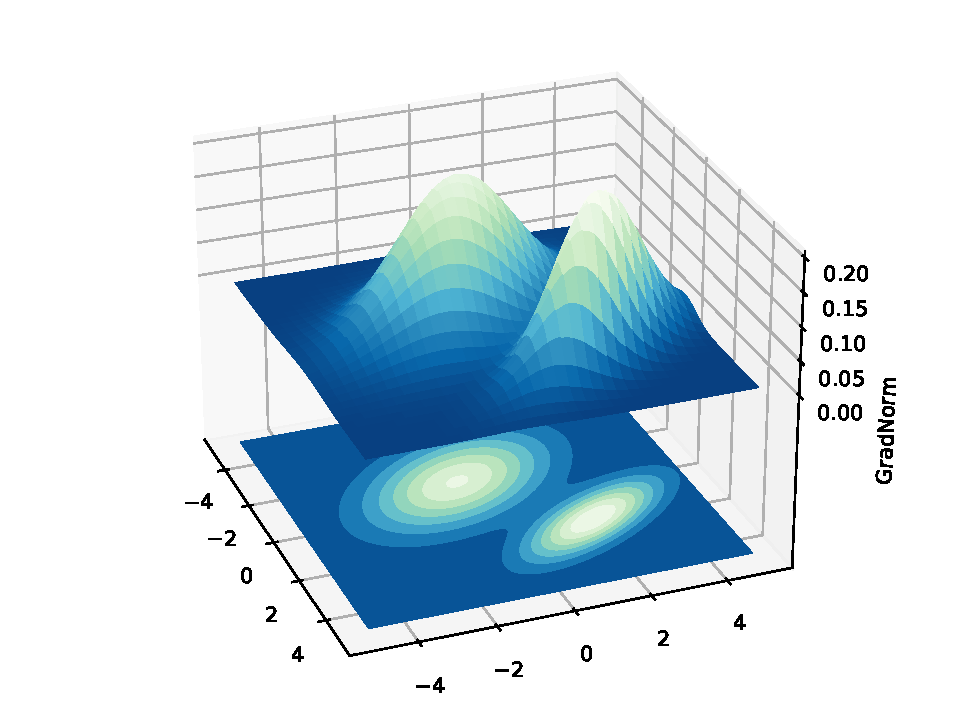
\includegraphics[width=0.45\textwidth]{figures/teaser_figure_new5.pdf}
        \vspace{-0.5cm}
    \caption{\small{An example of two-dimensional input space. Input data is depicted in the $xy$-plane, while gradient norm for each input is depicted in the $z$-dimension. The magnitude of gradients is higher for ID data ({\color{green}light green}) than that for OOD data ({\color{blue}deep blue}).}}
    \label{fig:teaser}
    \vspace{-1.5cm}
\end{wrapfigure}
\textbf{{GradNorm} as OOD score} For a given parameter $w$, the gradient of the above KL divergence is:
\begin{align}
    \frac{\partial D_\text{KL}(\*u~||~\text{softmax}(f(\*x))}{\partial w} = \frac{1}{C}\sum_{i=1}^C \frac{\partial \mathcal{L}_\text{CE}(f(\*x),i)}{\partial w},
\end{align}
where $w$ is a component of network parameter $\theta$. Notice that the gradient of the entropy term is $0$, \ie $\partial H(\*u) / \partial w=0$. In other words, the gradient of KL divergence is equivalent to averaging the derivative of the categorical cross-entropy loss for \emph{all} labels.

We now define the OOD score via a vector norm of gradients of the selected parameters:
\begin{equation}
\label{eq:score}
    S(\*x) = \lVert\frac{\partial D_\text{KL}(\*u~\lVert~\text{softmax}(f(\*x))}{\partial \*w}  \rVert_p,
\end{equation}
where $\lVert \cdot \rVert_p$ denotes $L_p$-norm and $\*w$ is the set of   parameters in vector form\footnote{We concatenate all selected parameters into a single vector regardless of the original shapes of the parameters.}. We term our method~\texttt{GradNorm}, short for gradient norm. In practice, ~\texttt{GradNorm} can be conveniently implemented by calculating the cross-entropy loss between the predicted softmax probability and a uniform vector as the target. We will discuss the choices and impacts of the selected parameter set $\*w$ in Section~\ref{sec:ablations}. 
% Depending on the selection of parameters $\*w$, 
% we investigate several variants of GradNorm with different heuristics to select parameters whose gradients will contribute to the final OOD score:

% \paragraph{All Layer} Gradients of all trainable parameters in all layers of the model will be included in calculating the vector norm. This requires a full backpropagation of the model.

% \paragraph{Block n} Gradients of all trainable parameters in all layers of the n-th block will be included in calculating the vector norm.

% \paragraph{Last Layer} Only the gradient of the weight parameter in the last linear layer will contribute to the OOD score. This is computationally more efficient because backpropagation only needs to be performed within the last layer.




\textbf{Rationale of {GradNorm}} Our operating hypothesis is that using the KL divergence for backpropagation, the gradient norm is higher for ID data than that for OOD data. As we show in Section~\ref{sec:ablations}, using the gradient norm of the KL divergence is more effective than using the KL divergence directly.
Moreover, \texttt{GradNorm} derived from the KL divergence with a uniform target offers two advantages over gradient norms derived from the standard cross-entropy loss.
% given below:
% \begin{equation}
%     \lVert\frac{\partial \mathcal{L}_\text{CE}(f(\*x),y)}{\partial \*w} \rVert.
% \end{equation}
\vspace{-0.2cm}
\begin{itemize}
\itemsep0em
    \item First, our method is \emph{label-agnostic} and does not require any ground-truth label. It can be flexibly used during inference time when the label is unavailable for either ID or OOD data. 
    \item  Second, it captures the \emph{uncertainty across all categories}, providing more information for OOD detection. We will provide empirical evidence to show the importance of utilizing all labels in Section~\ref{sec:ablations}.
\end{itemize}


% \subsection{Gradient as OOD Score}
% \label{sec:gradient_score}
% After backpropagation with the proposed CE loss with all-one vector, we obtain the gradient of each parameter $p$:
% \begin{equation}
%     G(p) = \frac{\partial \mathcal{L}}{\partial p}.
% \end{equation}

% Finally the gradients of all selected parameters will be condensed into an OOD score via a vector norm:
% \begin{equation}
%     S = \lVert G(\mathcal{P}) \rVert,
% \end{equation}
% where $\lVert \cdot \rVert$ can be any $L_p$-norm and $\mathcal{P}$ is the set of all selected parameters. We concatenate all selected parameters into a single vector regardless of the original shapes of the parameters. Note that since the positive norm is used as OOD score, an interpretation behind the scoring function is: larger gradients indicate in-distribution data while smaller gradients indicate OOD data.

% \subsection{Out-of-distribution Detection with Gradients}
% Scores from in-distribution and out-of-distribution inputs are obtained utilizing Algorithm~\ref{alg:scores}. These scores follow the methodology we described in Section 3.3, utilizing the input's gradients to derive a series of scores for each given input.

% \begin{algorithm}[ht]
%   \caption{Extracting Gradient Scores}
%   \label{alg:scores}
% \begin{algorithmic}
%   \STATE {\bfseries Input:} $model$, $testing\_set$, $T$
%   \STATE {\bfseries Output:} $scores$
%   \vskip 0.15cm
%   \STATE $scores = \{\}$
%   \FOR{$input$ in $training\_set$}
%   \STATE $label = ones(model(input).shape)$
%   \STATE $loss = BCE\_{loss}(input, label)$
%   \STATE $loss.backward()$
%   \STATE $scores \leftarrow ||inputs.grad.data||_1$
%   \ENDFOR
%   \STATE {\bfseries return} $scores$
% \end{algorithmic}
% \end{algorithm}

% Out-of-distribution detection, as a binary classification problem, utilizes a threshold $\gamma$ derived based on the in-distribution scores and out-of-distribution scores. This threshold can be derived empirically throughout multiple means \cite{chen2020, hendrycks2018, hendrycks2019, liu2020}. The final classification of an input can be computed utilizing Algorithm~\ref{alg:detection} in which the $threshold$ function can be any empirical estimate desired.

% \begin{algorithm}[ht]
%   \caption{Gradient Out-of-distribution Detection}
%   \label{alg:detection}
% \begin{algorithmic}
%   \STATE {\bfseries Input:} $model$, $x$, $T$, $in\_scores$, $out\_scores$
%   \STATE {\bfseries Output:} $classification$
%   \vskip 0.15cm
%   \STATE $\gamma = threshold(in\_scores, out\_scores)$
%   \STATE $label = ones(model(input).shape)$
%   \STATE $loss = BCE\_{loss}(x, label)$
%   \STATE $loss.backward()$
%   \STATE $score = ||x.grad.data||_1$
%   \IF{$score \geq \gamma$}
%   \STATE {\bfseries return} $in\_distribution$
%   \ELSE
%   \STATE {\bfseries return} $out\_distribution$
%   \ENDIF
% \end{algorithmic}
% \end{algorithm}


\vspace{-0.3cm}

\section{Experiments}
\label{sec:experiments}
\vspace{-0.3cm}
In this section, we evaluate \texttt{GradNorm} on a large-scale OOD detection benchmark with ImageNet-1k as in-distribution dataset~\cite{huang2021mos}. We describe experimental setup in Section~\ref{sec:exp_setup} and demonstrate the superior performance of \texttt{GradNorm} over existing approaches in Section~\ref{sec:ablations}, followed by extensive ablations and analyses that improve the understandings of our approach. %Our code and dataset will be released to facilitate reproducible research.
%\footnote{Public Github repository provided to facilitate reproducible research (\url{https://github.com/deeplearning-wisc/Gradient_OOD})}.

\vspace{-0.2cm}
\subsection{Experimental Setup}
\label{sec:exp_setup}
\vspace{-0.2cm}
\textbf{Dataset} 
We use the large-scale ImageNet OOD detection benchmark proposed by \citeauthor{huang2021mos}~\cite{huang2021mos}.
ImageNet benchmark is not only more realistic (with higher resolution images) but also more challenging (with a larger label space of 1,000 categories). 
We evaluate on four OOD test datasets, which are from subsets of \texttt{iNaturalist}~\cite{van2018inaturalist}, \texttt{SUN}~\cite{xiao2010sun}, \texttt{Places}~\cite{zhou2017places}, and \texttt{Textures}~\cite{cimpoi2014describing}, with non-overlapping categories \wrt ImageNet-1k (see Appendix~\ref{app:dataset} for detail). The evaluations span a diverse range of domains including fine-grained images, scene images, and textural images. We further evaluate on CIFAR benchmarks that are routinely used in literature (see Appendix~\ref{app:cifar}).
%We use the standard train/val splits for all datasets. %We use ImageNet-1k~\cite{deng2009imagenet} as the ID dataset. ImageNet-1k covers a wide range of real-world objects and has 10-100 times more labels compared to CIFAR datasets used in the prior literature. Additionally, the image resolution is significantly higher than CIFAR (32$\times$32) and MNIST (28$\times$28), making our evaluation more applicable for the real-world setting. 

% \vspace{-0.3cm}
% \paragraph{Out-of-distribution dataset}
% For ImageNet pre-trained model, we adopt the OOD test datasets in~\cite{huang2021mos} (see Appendix~\ref{app:ood_class} for concept list). Specifically, the four test OOD datasets are from (subsets of) \texttt{Places365}~\cite{zhou2017places}, \texttt{Textures}~\cite{cimpoi2014describing}, \texttt{iNaturalist}~\cite{van2018inaturalist}, and \texttt{SUN}~\cite{xiao2010sun} with non-overlapping categories w.r.t ImageNet. The evaluations span a diverse range of domains including fine-grained images, scene images, and textural images.
%To evaluate our approach, we consider a diverse collection of OOD datasets, spanning various domains including fine-grained images, scene images, and textural images. We carefully curate the OOD evaluation benchmarks to make sure concepts in these datasets are not overlapping with ImageNet-1k. Below we describe the construction of each evaluation dataset in detail. Samples of each OOD dataset are provided in Figure~\ref{fig:image_sample} in Appendix. For reproducibility, we provide the list of concepts chosen for each OOD dataset in Appendix~\ref{app:ood_class}. %\SL{compile appendix}

% \vspace{-0.2cm}
% \begin{itemize}
%     \item \textbf{iNaturalist}~\cite{van2018inaturalist} contains 859,000 plant and animal images organizable into over 5,000 different species. Each image is resized to have a max dimension of 800 pixels. We manually select 110 plant classes not present in ImageNet-1k, and randomly sample 10,000 images from these 110 classes.
%     \vspace{-0.1cm}
%     \item \textbf{SUN}~\cite{xiao2010sun} contains over 130,000 images of scenes with 397 categories. SUN and ImageNet-1k have overlapping categories. Therefore, we carefully select 50 nature-related concepts that are unique in SUN, such as \textit{forest} and \textit{iceberg}. We randomly sample 10,000 images from these 50 classes.
%     \vspace{-0.1cm}
%     \item \textbf{Places}~\cite{zhou2017places} is another scene dataset with similar concept coverage as SUN. A chosen subset of 10,000 images across 50 classes (not contained in ImageNet-1k) is used.
%     \vspace{-0.1cm}
%     \item \textbf{Textures}~\cite{cimpoi14describing} contains 5,640 real-world texture images under 47 categories. We use the entire dataset for evaluation.
% \end{itemize}

% \vspace{-0.2cm}
% \subsection{Experimental Setup}
% \label{sec:exp_setup}
% \vspace{-0.3cm}
\textbf{Model and hyperparameters} 
We use Google BiT-S models\footnote{\url{https://github.com/google-research/big_transfer}}~\cite{kolesnikov2020big} pre-trained on ImageNet-1k with a ResNetv2-101 architecture~\cite{he2016identity}. We report performance on an alternative architecture, DenseNet-121~\cite{huang2017densely}, in Section~\ref{sec:ablations}. %We fine-tune the top fully-connected (FC) layer from the BiT-S-R101x1 backbone with depth 101 and width factor 1. 
%We provide a comparison of varying model capacity in Section~\ref{sec:exp_results}. 
Additionally, we use $L_1$-norm-based OOD scores as the default and explore the effect of other $L_p$-norms in Section~\ref{sec:ablations}. The temperature parameter $T$ is set to be 1 unless specified otherwise, and we explore the effect of different temperatures in Section~\ref{sec:ablations}. At test time, all images are resized to 480 $\times$ 480.
%All experiments were performed on NVIDIA GeForce RTX 2080Ti GPUs. 

% \vspace{-0.3cm}
% \paragraph{Evaluation metrics} We measure the performance of our method for OOD detection based on (1) the false positive rate of the OOD inputs when the true positive rate of in-distribution inputs is 95\% (FPR95) and (2) the area under the receiver operating characteristic curve (AUROC). %Both metrics are commonly used in literature.

% \begin{figure}[t]
%     \centering
%     \includegraphics[width=0.5\textwidth]{figures/layer_wise_trend.pdf}
%     \caption{Layer-wise trend}
%     \label{fig:layer_wise_trend}
% \end{figure}


\begin{table*}[t]
\centering
\scriptsize{

\begin{tabular}{c|l|C{0.03\textwidth}C{0.045\textwidth}|C{0.03\textwidth}C{0.045\textwidth}|C{0.03\textwidth}C{0.045\textwidth}|C{0.03\textwidth}C{0.045\textwidth}|C{0.03\textwidth}C{0.045\textwidth}}
\toprule
\multirow{3}{*}{\textbf{\begin{tabular}[c]{@{}c@{}}Method\\ Space\end{tabular}}} & \multicolumn{1}{c|}{\multirow{3}{*}{\textbf{Method}}} & \multicolumn{2}{c|}{\textbf{iNaturalist}}    & \multicolumn{2}{c|}{\textbf{SUN}}            & \multicolumn{2}{c|}{\textbf{Places}}         & \multicolumn{2}{c|}{\textbf{Textures}}       & \multicolumn{2}{c}{\textbf{Average}}        \\ \cline{3-12} 
                                                                                      & \multicolumn{1}{c|}{}                                 & \tiny{FPR95}                & \tiny{AUROC}                 & \tiny{FPR95}                & \tiny{AUROC}              & \tiny{FPR95}                & \tiny{AUROC}                 & \tiny{FPR95}                & \tiny{AUROC}                 & \tiny{FPR95}                & \tiny{AUROC}               \\
                                                                                      & \multicolumn{1}{c|}{}                                 & \multicolumn{1}{c}{$\downarrow$} & \multicolumn{1}{c|}{$\uparrow$} & \multicolumn{1}{c}{$\downarrow$} & \multicolumn{1}{c|}{$\uparrow$} & \multicolumn{1}{c}{$\downarrow$} & \multicolumn{1}{c|}{$\uparrow$} & \multicolumn{1}{c}{$\downarrow$} & \multicolumn{1}{c|}{$\uparrow$} & \multicolumn{1}{c}{$\downarrow$} & \multicolumn{1}{c}{$\uparrow$}  \\ \midrule
                                
\multirow{3}{*}{Output}                                                         & MSP\tiny{~\cite{hendrycks2016baseline}}                                                   & 63.69                & 87.59                 & 79.98                & 78.34                 & 81.44                & 76.76                 & 82.73                & 74.45                 & 76.96                & 79.29                \\
                                                                                      & ODIN\tiny{~\cite{liang2018enhancing}}                                                  & 62.69                & 89.36                 & 71.67                & 83.92                 & 76.27                & 80.67                 & 81.31                & 76.30                 & 72.99                & 82.56                \\
                                                                                    %   & Generalized ODIN$^\clubsuit$ \tiny{~\cite{hsu2020generalized}}                                      & 66.36                & 84.68                 & 62.17                & 85.98                 & 66.83                & 83.38                 & 67.00                & \textbf{81.23}                 & 65.59                & 83.82                \\
                                                                                      & Energy\tiny{~\cite{liu2020energy}}                                                & 64.91                & 88.48                 & 65.33                & 85.32                 & 73.02                & 81.37                 & 80.87                & 75.79                 & 71.03                & 82.74                \\
                                                                                      %& \tiny{MC-Dropout~\cite{gal2016dropout}}                                            & 74.90 &	82.64 &	77.27 &	77.27 &	82.38 &	73.46 &	84.70 &	70.30 &	79.81 &	75.92       \\ 
                                                                                      \midrule
Feature                                                                         & Mahalanobis\tiny{~\cite{lee2018simple}}                                            & 96.34                & 46.33                 & 88.43                & 65.20                 & 89.75                & 64.46                 & \textbf{52.23}                & 72.10                 & 81.69                & 62.02                \\ \midrule
\multirow{1}{*}{Gradient}                    
                                                                                      & \textbf{GradNorm (ours)}                              & \textbf{50.03}       & \textbf{90.33}        & \textbf{46.48}       & \textbf{89.03}        & \textbf{60.86}       & \textbf{84.82}        & 61.42                & \textbf{81.07}                 & \textbf{54.70}       & \textbf{86.31}       \\ \bottomrule
\end{tabular}
}
\caption{\small{\textbf{Main Results.} OOD detection performance comparison between \texttt{GradNorm} and baselines. All methods utilize the standard ResNetv2-101 model trained on ImageNet~\cite{deng2009imagenet}. The classification model is trained on {ID data only}.
$\uparrow$ indicates larger values are better, while $\downarrow$ indicates smaller values are better. All values are percentages. %$\clubsuit$ indicates that retraining of the classification model is required under a different loss function. 
All methods are post hoc and can be directly used for pre-trained models.}}
%\SL{add missing baselines. Is there any argument on why Generalized ODIN is not a fair comparison?}}
\label{table:main}
\vspace{-0.4cm}
\end{table*}

\vspace{-0.2cm}
\subsection{Results and Ablation Studies}
\label{sec:ablations}
\vspace{-0.2cm}
\textbf{Comparison with output- and feature-based methods} 
The results for ImageNet evaluations are shown in Table~\ref{table:main}, where \texttt{GradNorm} demonstrates  superior performance. We report OOD detection performance for each OOD test dataset, as well as the average over the four datasets. For a fair comparison, all the methods use the same pre-trained backbone, without regularizing with auxiliary outlier data. 
% The results for ImageNet pre-trained model are shown in Table~\ref{table:main}, where we report performance for each OOD test dataset as well as the average performance. For fair evaluation, we compare \texttt{GradNorm} with competitive methods that are based on discriminative models. 
%It is important to note that generative models~\cite{hinz2018generating} can be prohibitively challenging to train and optimize on large-scale real-world datasets. 
In particular, we compare with MSP~\cite{hendrycks2016baseline}, ODIN~\cite{liang2018enhancing}, Mahalanobis~\cite{lee2018simple}, as well as Energy~\cite{liu2020energy}.
%Among those, MSP and energy score are hyperparameter-free approaches.  
%For all methods, we derive OOD scoring functions from the same network trained on in-distribution data without exposure to auxiliary outlier data, because it can be prohibitive to construct an auxiliary outlier dataset in large-scale image classification. 
\emph{Details and hyperparameters of baseline methods can be found in Appendix~\ref{app:baseline}}. %While some baselines such as ~\cite{liang2018enhancing, lee2018simple} may require validation datasets, \texttt{GradNorm} is hyperparameter free and can be used in OOD-agnostic setting. 

\texttt{GradNorm} outperforms the best output-based baseline, Energy score~\cite{liu2020energy}, by \textbf{16.33}\% in FPR95. \texttt{GradNorm} also outperforms a competitive feature-based method, Mahalanobis~\cite{lee2018simple}, by \textbf{26.99}\% in FPR95. We hypothesize that the increased size of label space makes the class-conditional Gaussian density estimation less viable. It is also worth noting that significant overheads can be introduced by some methods. 
%For instance, Generalized ODIN~\cite{hsu2020generalized} is not a post hoc method, as it requires retraining the model using a different DeConf loss function and hence is less convenient compared to \texttt{GradNorm} and other post hoc baselines. 
For instance, Mahalanobis~\cite{lee2018simple} requires collecting feature representations from intermediate layers over the entire training set, which is expensive for large-scale datasets such as ImageNet. 
%Methods such as \cite{hsu2020generalized}, \cite{lee2018simple} and \cite{liang2018enhancing} also require hyper-parameter tuning on a validation dataset. 
In contrast, \texttt{GradNorm} can be conveniently used through a simple gradient calculation without hyper-parameter tuning or additional training.
% Moreover, some methods require training a separate binary classifier~\cite{lee2018simple} or retraining the classification model under a different loss function~\cite{hsu2020generalized}, whereas \texttt{GradNorm} can be conveniently used through a simple threshold comparison.   




% %\vspace{-0.1cm}
% \textbf{Comparison with previous gradient-based method}
% \citeauthor{lee2020gradients}~\cite{lee2020gradients} proposed an OOD detection framework using the $L_2$-norm of gradients. Importantly, they do not directly use gradient norms for OOD detection, but instead, use them as the input for training a separate binary classifier. Furthermore, the binary classifier is trained on the OOD datasets, which can unfairly overfit to the test data and does not suit OOD-agnostic settings in the real world. In contrast, our methodology mitigates the shortcomings in that \texttt{GradNorm} (1) does not require any new model training, (2) is hyperparameter-free, and (3) is suitable for OOD-agnostic settings. 
% %In fact, our experiments suggest that the performance of \citeauthor{lee2020gradients}'s method is very limited when no prior knowledge about OOD data is available. 


% We compare the performance of \texttt{GradNorm} with their approach in Table~\ref{table:compare_with_lee_alregib}. For a fair comparison, we do not use any OOD data for both methods. %For \citeauthor{lee2020gradients}'s method, we use the gradients of uniform noise as a surrogate of OOD data to train the binary classifier. 
% \texttt{GradNorm} reduces the FPR95 by \textbf{15.45}\% compared with their approach. % in a fair comparison where no OOD data can be used in training for both methods.
% Additionally, our work comprehensively investigates and explains various important design choices in using gradient-based methods (see Section~\ref{sec:ablations}), which is otherwise not considered in \cite{lee2020gradients}. %Furthermore, different from \citeauthor{lee2020gradients}, our evaluation is based on high-resolution large-scale datasets, which makes our results more relevant for the real world.



%All these methods rely on pre-trained networks with the same architecture, ResNetv2-101. For comprehensive evaluation, in Appendix~\ref{app:densenet} we report the performance on another pre-trained network, DenseNet-121, on which \texttt{GradNorm} remains superior to all baseline methods.

% Our main results are based on gradient norm extracted from weight parameters in the last layer. We further ablate the performance of \texttt{GradNorm} with different selection of gradients.
%In Table~\ref{table:main}, we compare the performance of our approach with existing approaches on all four OOD datasets as well as the average performance. We report the performance of Last Layer and we will compare the performance of all different variants of GradNorm in Section~\ref{sec:layer_ablation}.

% For fair comparison, we compare with competitive methods in the literature that derive OOD scores from a model trained on in-distribution data only and do not rely on any auxiliary outlier data, and all methods utilize the same pre-trained ResNetv2-101 model to generate OOD scores. GradNorm introduces significant improvements over baseline methods, reducing the average FPR95 by \textbf{16.33\%} compared to the best baseline.

% All Layer achieves quite comparable performance with previous methods and reduces the average FPR95 by \textbf{1.68\%} compared to the best baseline approach. Meanwhile, Last Layer not only is computationally more efficient, but also introduces significant improvements over baseline methods and All Layer, reducing the average FPR95 by \textbf{16.33\%} compared to the best baseline.
%\subsubsection{How do other $L_p$-norms affect OOD detection performance?}
%\label{sec:norm_ablation}

% To condense the information extracted from the gradient space, we've chosen to solve for the magnitude of the gradient through its Manhattan distance ($L_1$-norm). However, as proposed by \citeauthor{lee2020gradients}, the Euclidean distance ($L_2$-norm) of the gradients also presents an effective method for condensing gradient information. In this ablation we aim to compare the OOD detection performance under different $L_p$-norms.

% We use CE loss with all-one vector for backpropagation and gradients are extracted only from the last layer parameters. The OOD detection performance of $L_{1 \sim 5}$-norm and $L_{\infty}$-norm is shown in Figure~\ref{fig:norm_ablation}. $L_1$-norm always introduces the best OOD detection performance on all four datasets, while the performance under other norms is drastically worse.

% \subsubsection{How gradients from different layers affect OOD detection performance}



%For a more comprehensive analysis, we also report the performance of \citeauthor{lee2020gradients}'s method under $L_1$-norm in Table~\ref{tab:al_norm_ablation} in Appendix. Interestingly, using $L_1$-norm instead of $L_2$-norm also introduces a significant performance boost for their method, reducing the FPR95 by 35.73\%.



%\vspace{-0.2cm}
% \subsection{Ablation Studies}
% \label{sec:ablations}
\paragraph{Gradients from the last layer is sufficiently informative} 
In this ablation, we investigate several variants of \texttt{GradNorm} where the gradients are extracted from different network depths. Specifically, we consider gradients of (1) \textbf{block n}: all trainable parameters in the $n$-th block, (2) \textbf{all parameters}: all trainable parameters from all layers of the network, %will be included in calculating the vector norm which requires a full backpropagation of the model, 
and (3) \textbf{last layer parameters}: weight parameters from the last fully connected (FC) layer. 


\begin{wraptable}{r}{0.4\textwidth}
% \vspace{-0.3cm}
{\footnotesize{
\begin{tabular}{c|cc}
\toprule
\multirow{2}{*}{\textbf{\begin{tabular}[c]{@{}c@{}}Gradient\\ Space\end{tabular}}} & \textbf{FPR95}       & \textbf{AUROC}     \\
                                                                                       & \multicolumn{1}{c}{$\downarrow$} & \multicolumn{1}{c}{$\uparrow$}  \\ \midrule
%Output   & 71.03  & 82.74 \\
Block 1                                                                                & 73.52                & 76.41                \\
Block 2                                                                                & 74.34                & 76.63                \\
Block 3                                                                                & 71.73                & 78.11                \\
Block 4                                                                                & 65.07                & 85.11                \\
All params                                                                              & 69.35                & 81.14                \\
Last layer params                                                                             & \textbf{54.70}       & \textbf{86.31}       \\ \bottomrule
\end{tabular}}
}
    \caption{\small{Effect of \texttt{GradNorm} using different subset of gradients. Gradient norm derived from deeper layers yield better OOD detection performance.}}
    \label{tab:block_trend_ablation}
    % \vspace{-0.3cm}
\end{wraptable}

Table~\ref{tab:block_trend_ablation} contrasts the OOD detection performance using different \emph{gradient space}. For each setting, we report the FPR95 and AUROC averaged across four OOD datasets. We observe that gradients from deeper layers tend to yield significantly better performance than shallower layers. This is desirable since gradients \wrt deeper layers are computationally more efficient than shallower layers. Interestingly,\texttt{GradNorm} obtained from the last linear layer yield the best results among all variants. Practically, one only needs to perform backpropagation \wrt the last linear layer, which incurs negligible computations. Therefore, our main results are based on the norm of gradients extracted from weight parameters in the last FC layer of the neural network. 






%In contrast, methods such as ODIN~\cite{liang2018enhancing} and ~\citeauthor{lee2020gradients} require a full backpropagation, resulting in slow inference. %While the performance of early layers is not stable, the last several layers tend to produce better performance. More importantly, OOD scores obtained from the last linear layer always yield near-optimal (if not the best) results among all layers. Meanwhile, in practice, using gradients from only the very last layer is also very desirable because it avoids large overhead of backpropagating all the way to early layers.

%  More importantly, Last Layer yields the optimal performance among all these variants, indicating we only need to perform backpropagation within the last linear layer in practice.

% \paragraph{All Layer} Gradients of all trainable parameters in all layers of the model will be included in calculating the vector norm. This requires a full backpropagation of the model.

% \paragraph{Block n} Gradients of all trainable parameters in all layers of the n-th block will be included in calculating the vector norm.

% \paragraph{Last Layer} Only the gradient of the weight parameter in the last linear layer will contribute to the OOD score. This is computationally more efficient because backpropagation only needs to be performed within the last layer.


%In Section~\ref{sec:gradient_score} we proposed several heuristic approaches to select the set of parameters $\mathcal{P}$ whose gradients will contribute to the final OOD score, All Layer, Block n and Last Layer. %In this ablation we aim to compare the performance of different selections and also hopefully provide an upper bound of gradient-based OOD detection.








\vspace{-0.2cm}
\paragraph{{GradNorm} with one-hot v.s. uniform targets}



In this ablation, we contrast \texttt{GradNorm} derived using uniform targets (ours) v.s. one-hot targets. Specifically, our scoring function Equation~\ref{eq:score}  is equivalent to 
\begin{align}
    S(\*x) = \lVert \frac{1}{C}\sum_{i=1}^C \frac{\partial \mathcal{L}_\text{CE}(f(\*x),i)}{\partial \*w} \rVert,
\end{align}
which captures the gradient of cross-entropy loss across \emph{all} labels. In contrast, we compare against an alternative scoring function that utilizes \emph{only one} dominant class label:
\begin{align}
    S_\text{one-hot}(\*x) = \lVert \frac{\partial \mathcal{L}_\text{CE}(f(\*x),\hat y)}{\partial \*w} \rVert,
\end{align}
where $\hat y$ is the predicted class with the largest output. 

%For traditional CE loss with one-hot vector, we use the negative $L_1$-norm as OOD score, since gradient magnitude of in-distribution data tend to be higher. 
%Results suggest that traditional cross-entropy loss has very limited capabilities in distinguishing between in- v.s. out-of-distribution data and that our CE loss with all-one vector beats traditional CE loss with one-hot vector by a large margin. 


\begin{figure*}[t]
    \centering
        \begin{subfigure}[b]{1.0\textwidth}
        \centering
        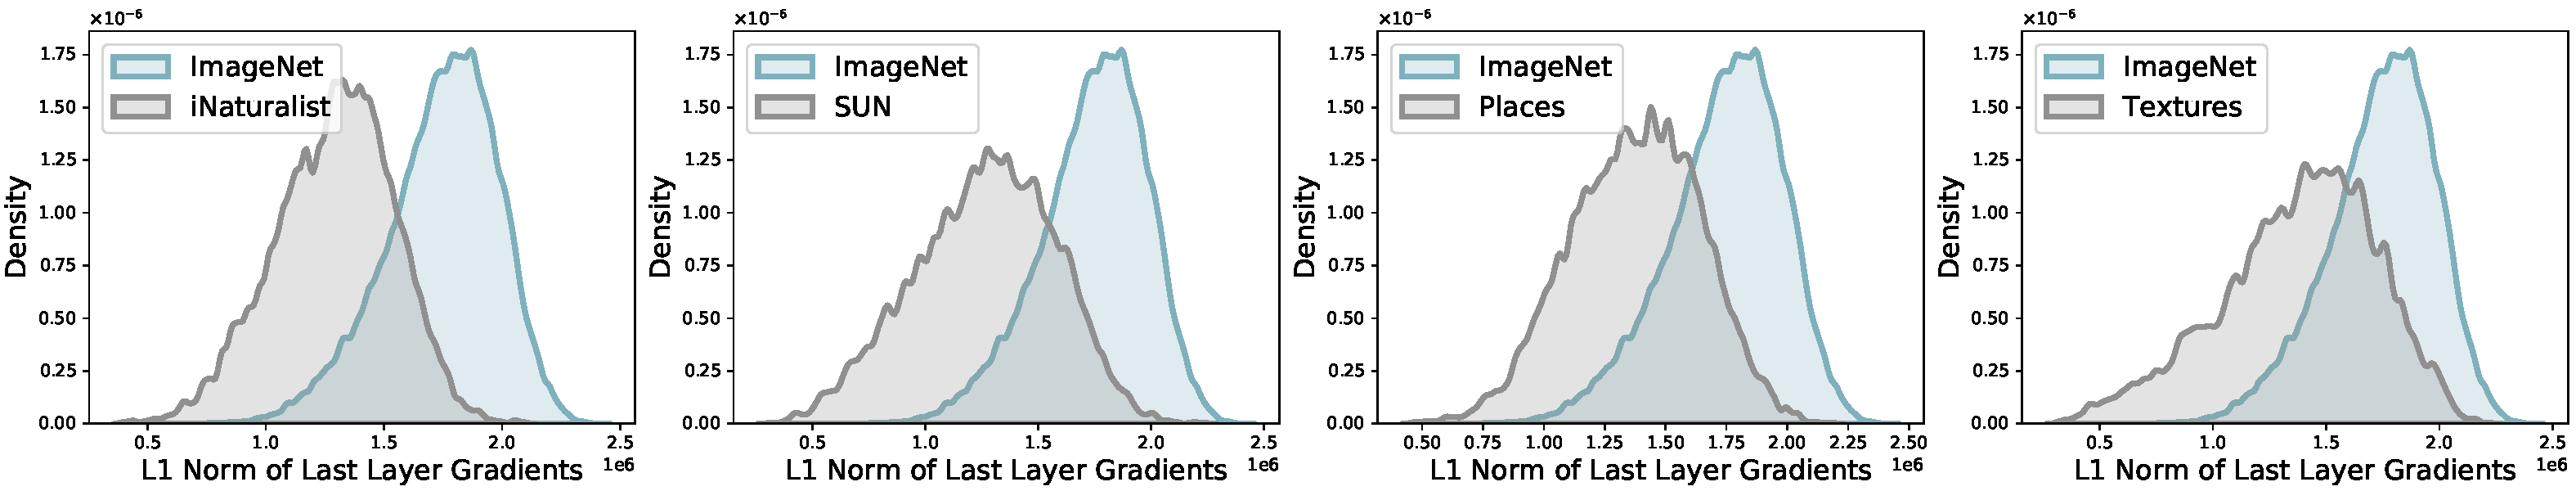
\includegraphics[width=1.0\textwidth]{figures/our_ce_distribution_final.pdf}
        \caption{Gradient norms using KL divergence between the softmax prediction and the \textbf{uniform} target.}
        \label{subfig:score_dist_uniform}
        \end{subfigure}
        \begin{subfigure}[b]{1.0\textwidth}
        \centering
        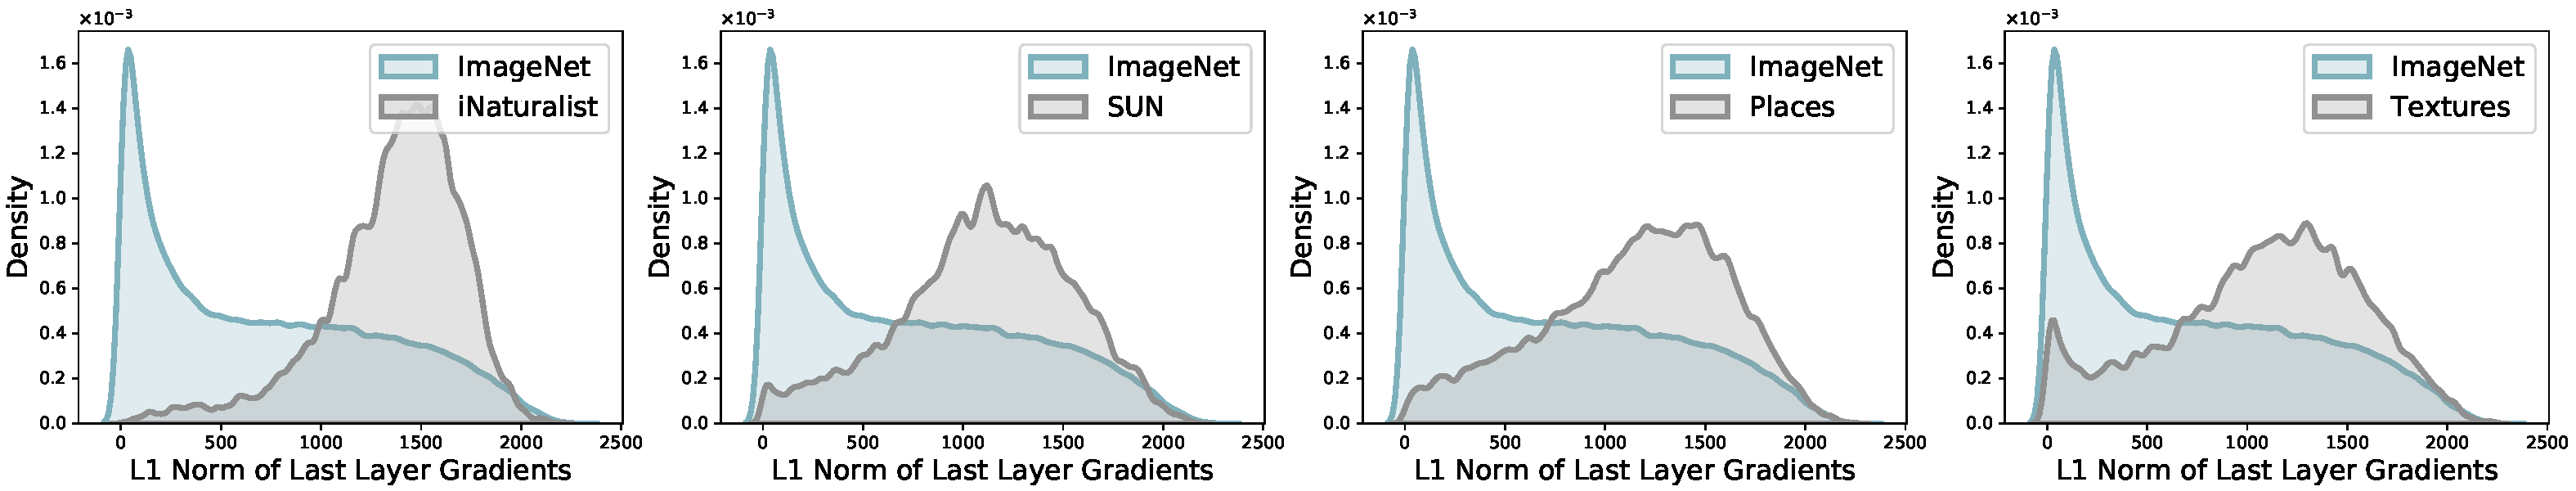
\includegraphics[width=1.0\textwidth]{figures/original_ce_distribution_final.pdf}
        \caption{Gradient norms using KL divergence between the softmax prediction and the \textbf{one-hot} target.}
        \label{subfig:score_dist_onehot}
        \end{subfigure}
    \caption{\small{Comparison of $L_1$-norm distributions of last layer gradients between KL divergence with \emph{uniform} target and KL divergence with \emph{one-hot} target. We show in-distribution data in green and OOD data in gray. }}
    \label{fig:score_dist}
    \vspace{-0.4cm}
\end{figure*}

We first analyze the score distributions using uniform targets (\textbf{top}) and one-hot targets (\textbf{bottom}) for ID and OOD data in Figure~\ref{fig:score_dist}. 
There are two salient observations we can draw: (1) using uniform target (ours), gradients of ID data indeed have larger magnitudes than those of OOD data, as the softmax prediction tends to be less uniformly distributed (and therefore results in a larger KL divergence). In contrast, the gradient norm using one-hot targets shows the opposite trend, with ID data having lower magnitudes. This is also expected since the training objective explicitly minimizes the cross-entropy loss, which results in smaller gradients for the majority of ID data. (2) The score distribution using one-hot targets displays a strong overlapping between ID (green) and OOD (gray) data, with large variances. In contrast, our method \texttt{GradNorm} can significantly improve the separability between ID and OOD data, resulting in better OOD detection performance.


\begin{wrapfigure}{r}{0.48\textwidth}
\vspace{-0.6cm}
    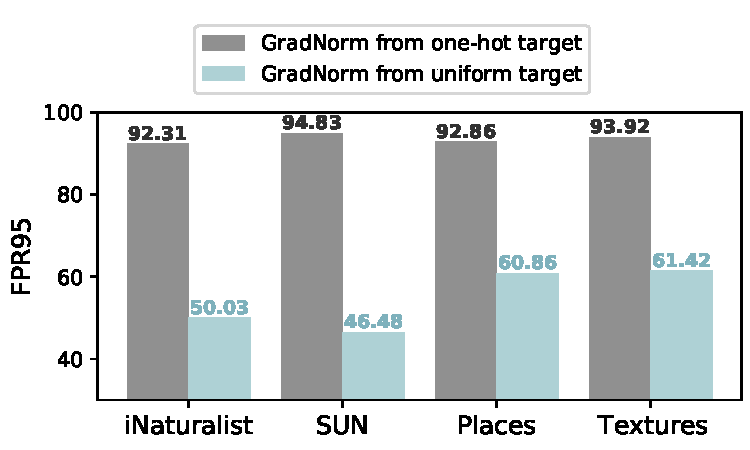
\includegraphics[width=0.45\textwidth]{figures/traditional_ce_fpr95_green.pdf}
    \caption{\small{OOD detection performance (FPR95) comparison between uniform (ours) v.s. one-hot target.}}
    \vspace{-0.4cm}
    \label{fig:traditional_ce_fpr95}
\end{wrapfigure}



Figure~\ref{fig:traditional_ce_fpr95} reports the OOD detection performance using uniform targets (ours) v.s. one-hot targets. We use $L_1$-norm in both cases. For one-hot targets, we use the negative norm, \ie $-S_\text{one-hot}(\*x)$, to align with the convention that ID data has higher scores. \texttt{GradNorm} with uniform targets outperforms its counterpart with one-hot targets by a large margin. For instance, \texttt{GradNorm} reduces FPR95 by \textbf{48.35}\% when evaluated on the SUN dataset. Our analysis signifies the importance of measuring OOD uncertainty using all label information.

% but are larger than OOD data under CE loss with all-one vector. Second, under traditional CE loss with a one-hot vector, gradients from in- and out-of-distribution data share a wide range of overlapping. However, under CE loss with all-one vector, the variance of gradient distributions for both in- and out-of-distribution data significantly decreases, and the overlapping range between in- and out-of-distribution data is narrowed. 



% \vspace{-0.2cm}
\paragraph{GradNorm is effective on alternative neural network architecture} We evaluate \texttt{GradNorm} on a different architecture DenseNet-121~\cite{huang2017densely}, and report performance in Table~\ref{tab:densenet}. \texttt{GradNorm} is consistently effective, outperforming the best baseline, Energy~\cite{liu2020energy}, by \textbf{10.29}\% in FPR95. 


\begin{table}[h]
    \centering
\scriptsize{
\begin{tabular}{c|l|C{0.03\textwidth}C{0.045\textwidth}|C{0.03\textwidth}C{0.045\textwidth}|C{0.03\textwidth}C{0.045\textwidth}|C{0.03\textwidth}C{0.045\textwidth}|C{0.03\textwidth}C{0.045\textwidth}}
\toprule
\multirow{3}{*}{\textbf{\begin{tabular}[c]{@{}c@{}}Method\\ Space\end{tabular}}} & \multicolumn{1}{c|}{\multirow{3}{*}{\textbf{Method}}} & \multicolumn{2}{c|}{\textbf{iNaturalist}}    & \multicolumn{2}{c|}{\textbf{SUN}}            & \multicolumn{2}{c|}{\textbf{Places}}         & \multicolumn{2}{c|}{\textbf{Textures}}       & \multicolumn{2}{c}{\textbf{Average}}        \\ \cline{3-12} 
                                                                                 & \multicolumn{1}{c|}{}                                 & \tiny{FPR95}                & \tiny{AUROC}                 & \tiny{FPR95}                & \tiny{AUROC}              & \tiny{FPR95}                & \tiny{AUROC}                 & \tiny{FPR95}                & \tiny{AUROC}                 & \tiny{FPR95}                & \tiny{AUROC}               \\
                                                                                      & \multicolumn{1}{c|}{}                                 & \multicolumn{1}{c}{$\downarrow$} & \multicolumn{1}{c|}{$\uparrow$} & \multicolumn{1}{c}{$\downarrow$} & \multicolumn{1}{c|}{$\uparrow$} & \multicolumn{1}{c}{$\downarrow$} & \multicolumn{1}{c|}{$\uparrow$} & \multicolumn{1}{c}{$\downarrow$} & \multicolumn{1}{c|}{$\uparrow$} & \multicolumn{1}{c}{$\downarrow$} & \multicolumn{1}{c}{$\uparrow$}  \\ \midrule
\multirow{3}{*}{Output}                                                          & MSP\tiny{~\cite{hendrycks2016baseline}}                                                   & 48.55                & 89.16                 & 69.39                & 80.46                 & 71.42                & 80.11                 & 68.51                & 78.69                 & 64.47                & 82.11                \\
                                                                                 & ODIN\tiny{~\cite{liang2018enhancing}}                                                  & 37.00                & 93.29                 & 57.30                & 86.12                 & 61.91                & 84.14                 & 56.49                & 84.62                 & 53.18                & 87.04                \\
                                                                                %  & Generalized ODIN$^\clubsuit$\tiny{~\cite{hsu2020generalized}}                                      & 63.41                & 85.38                 & 78.15                & 76.45                 & 76.11                & 77.41                 & 68.78                & 78.82                 & 71.61                & 79.52                \\
                                                                                 & Energy\tiny{~\cite{liu2020energy}}                                                & 36.39                & 93.29                 & 54.91                & 86.53                 & 59.98                & \textbf{84.29}        & 53.87                & 85.07                 & 51.29                & 87.30                \\ \midrule
Feature                                                                          & Mahalanobis\tiny{~\cite{lee2018simple}}                                           &  97.36 &	42.24 &	98.24 &	41.17 &	97.32 &	47.27 &	62.78 &	56.53 &	88.93 &	46.80                 \\ \midrule
 \multirow{1}{*}{Gradient}                                                      
%  & \citeauthor{lee2020gradients}\tiny{~\cite{lee2020gradients}}                                        &    74.97 &	62.39 &	43.59 &	\textbf{88.53} &	55.50 &	82.98 &	60.29 &	70.35 &	58.59 &	76.06      \\
                                                                                 & \textbf{GradNorm (ours)}                              & \textbf{23.87}       & \textbf{93.97}        & \textbf{43.04}       & \textbf{87.79}        & \textbf{53.92}       & 83.04                 & \textbf{43.16}       & \textbf{87.48}        & \textbf{41.00}       & \textbf{88.07}       \\ \bottomrule
\end{tabular}
}
    \caption{\small OOD detection performance comparison on a different architecture, \textbf{DenseNet-121}~\cite{huang2017densely}. Model is trained on ImageNet-1k~\cite{deng2009imagenet} as the ID dataset. %$\clubsuit$ indicates that retraining of the classification model is required under a different loss function. 
    All methods are post hoc and can be directly used for pre-trained models.}
    \label{tab:densenet}
    % \vspace{-0.5cm}
\end{table}




% \subsubsection{How do different model capacities affect OOD detection performance}
% \label{sec:capacity_ablation}



% \vspace{-0.2cm}

% \begin{wrapfigure}{r}{0.45\textwidth}
%     \includegraphics[width=0.45\textwidth]{gradient_ood_nips/figures/all_norm_fpr95_new.pdf}
%     \caption{\small{OOD detection performance comparison (FPR95) under different $L_p$-norms.}}
%     \label{fig:norm_ablation}
%     \vspace{-0.4cm}
% \end{wrapfigure}


\vspace{-0.2cm}
\paragraph{$L_1$-norm is the most effective} How does the choice of $L_p$-norm in Equation~\ref{eq:score} affect the OOD detection performance? To understand this, we show in Figure~\ref{fig:norm_ablation} the comparison using $L_{1 \sim 4}$-norm, $L_{\infty}$-norm, as well as the fraction norm (with $p=0.3$). 
%In particular, $L_1$-norm is the most effective metric in condensing information extracted from the \emph{gradient space}, achieving the best OOD detection performance on all four datasets. Critically, our analysis suggests that $L_2$-norm can result in up to a \textbf{22.13}\% rise in FPR95 compared to $L_1$-norm in our method. 
Compared with higher-order norms, $L_1$-norm achieves the best OOD detection performance on all four datasets. We hypothesize that $L_1$-norm is better suited since it captures information equally from all dimensions in the gradient space, whereas higher-order norms will unfairly highlight larger elements rather than smaller elements (due to the effect of the exponent $p$). In the extreme case, $L_{\infty}$-norm only considers the largest element (in absolute value) and results in the worst OOD detection performance among all norms. 
On the other hand, the fraction norm overall does not outperform $L_1$-norm. \emph{We additionally provide results for more $L_p$-norms in Appendix~\ref{app:more_norm}, with $p=\{0.3, 0.5, 0.8, 1,2,3,4,5,6,\infty\}$}. 


\begin{figure}[h]
    \centering
    % \vspace{-0.1cm}
    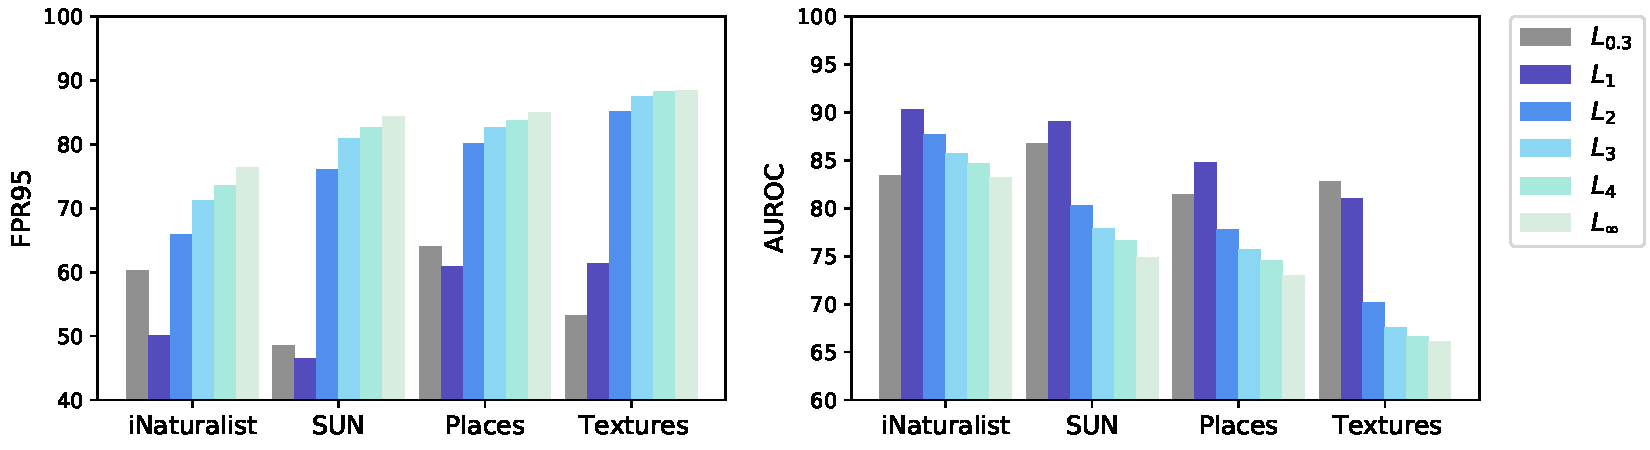
\includegraphics[width=0.99\textwidth]{figures/all_norm_fpr95_auroc.pdf}
    \caption{\small{OOD detection performance comparison under different $L_p$-norms. We show FPR95 (\emph{left}) and AUROC (\emph{right}).}}
    % \vspace{-0.1cm}
    \label{fig:norm_ablation}
\end{figure}

%\vspace{-0.2cm}

% \begin{wraptable}{r}{0.52\textwidth}
% \vspace{-0.4cm}
% {\footnotesize{
% \begin{tabular}{c|c|cc}
% \toprule
% \multirow{2}{*}{\textbf{Method}} & \multirow{2}{*}{\textbf{\begin{tabular}[c]{@{}c@{}}Method\\ Space\end{tabular}}} & \textbf{FPR95}       & \textbf{AUROC}       \\
%                                  &                                                                                  & \multicolumn{1}{c}{$\downarrow$} & \multicolumn{1}{c}{$\uparrow$} \\ \midrule
% KL divergence                    & Output                                                                           & 71.03                & 82.74                \\
% \texttt{GradNorm} of KL                       & Gradient                                                                         & \textbf{54.70}       & \textbf{86.31}       \\ \bottomrule
% \end{tabular}
% }}
%     \caption{\small{Comparison between \texttt{GradNorm} v.s. directly using the KL divergence as OOD scoring function.}}
%     \label{tab:kl_ablation}
%     \vspace{-0.3cm}
% \end{wraptable}



% \vspace{-0.2cm}
\textbf{Effect of temperature scaling} We evaluate our method \texttt{GradNorm} with different temperatures $T$ from $T=0.5$ to $T=1024$. As shown in Figure~\ref{fig:temper_ablation}, $T=1$ is optimal, while either increasing or decreasing the temperature will degrade the performance. This can be explained mathematically via the $V$ term in Equation~\ref{eq:decomp}. Specifically, using a large temperature will result in a smoother softmax distribution, with $C \cdot \frac{e^{f_j / T}}{\sum_{j=1}^C e^{{f_{j}} / T}}$ closer to 1 (and $V\rightarrow 0$). This leads to a less distinguishable distribution between ID and OOD. Our method can be hyperparameter-free by setting $T=1$. For completeness, we have included numerical results under a wider range of $T$ in Appendix~\ref{app:more_temper}.


\begin{figure}[h]
\centering
    \vspace{-0.2cm}
    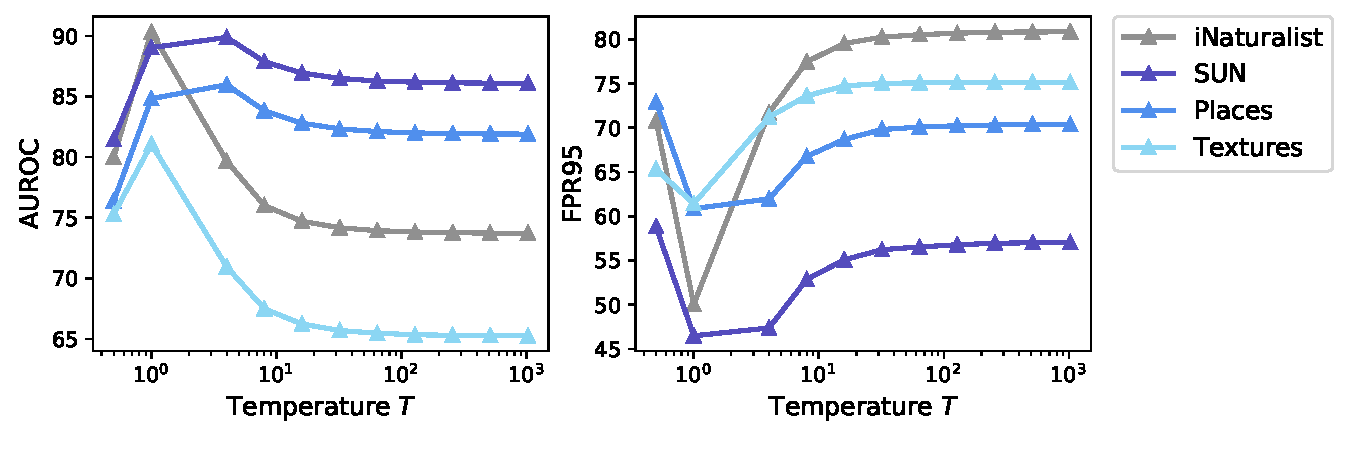
\includegraphics[width=0.95\textwidth]{figures/temperature_trend_new.pdf}
    % \vspace{-0.2cm}
    \caption{\small{OOD detection performance of \texttt{GradNorm} with varying temperature parameter $T$. We show AUROC (\emph{left}) and FPR95 (\emph{right}).}}
    \label{fig:temper_ablation}
    % \vspace{-0.5cm}
\end{figure}

\begin{wrapfigure}{r}{0.45\textwidth}
\vspace{-1.5cm}
    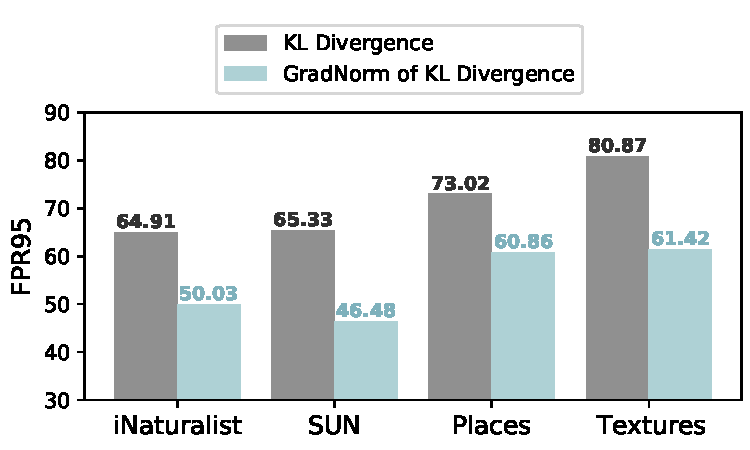
\includegraphics[width=0.43\textwidth]{figures/direct_kl_vs_gradnorm.pdf}
    \vspace{-0.3cm}
    \caption{\small{Comparison between \texttt{GradNorm} v.s. directly using the KL divergence as scoring function.}}
    \vspace{-0.5cm}
    \label{fig:kl_ablation}
\end{wrapfigure}

\vspace{-0.2cm}
\paragraph{{GradNorm} is more effective than directly using KL divergence} We provide an ablation, contrasting the performance of using \texttt{GradNorm} v.s. using the KL divergence derived from Equation~\ref{eq:kl} as OOD scoring function. The results are show in Figure~\ref{fig:kl_ablation}, where \texttt{GradNorm} yields significantly better performance than the KL divergence directly extracted from the \emph{output space}, demonstrating the superiority of \emph{gradient space} for OOD detection.


\begin{wraptable}{r}{0.4\textwidth}
\vspace{-0.3cm}
    \centering
\footnotesize{
\begin{tabular}{c|cc}
\toprule
\multirow{2}{*}{\textbf{\begin{tabular}[c]{@{}c@{}}Model Size\\ (depth x width)\end{tabular}}} & \textbf{FPR95}          & \textbf{AUROC}            \\
                                                                                                      & \multicolumn{1}{c}{$\downarrow$}     & \multicolumn{1}{c}{$\uparrow$}\\ \midrule
50x1                                                                                                  & 56.91          & 84.17  \\
101x1                                                                                                 & \textbf{55.84} & \textbf{84.63} \\
50x3                                                                                                  & 61.74          & 81.89 \\
152x2                                                                                                 & 61.76          & 81.33  \\
101x3                                                                                                 & 66.20          & 78.89 \\ \bottomrule
\end{tabular}
}
\caption{\small{OOD detection performance as the model capacity increases.}}
\label{tab:arch_ablation}
\vspace{-0.2cm}
\end{wraptable}

\paragraph{Effect of model capacity} In this ablation, we explore the OOD detection performance of \texttt{GradNorm} with varying model capacities. For the ease of experiments, we directly use Google BiT-S models pre-trained on ImageNet-1k~\cite{deng2009imagenet}. We compare the performance of the following model family (in increasing size): BiT-S-R50x1, BiT-S-R101x1, BiT-S-R50x3, BiT-S-R152x2, BiT-S-R101x3. All models are ResNetv2 architectures with varying depths and width factors. The average performance on 4 OOD datasets is reported in Table~\ref{tab:arch_ablation}. OOD detection performance is optimal when the model size is relatively small (ResNetv2-101x1), while further increasing model capacity will degrade the performance. Our experiments suggest that overparameterization can make gradients less distinguishable between ID and OOD data and that \texttt{GradNorm} is more suitable under a mild model capacity.% and that GradNorm doesn't rely on large model capacities to achieve good performance.





% \vspace{-0.2cm}
% \paragraph{Smaller model capacity benefits \texttt{GradNorm}} In this ablation, we explore the OOD detection performance of \texttt{GradNorm} with varying model capacities. For the ease of experiments, we directly use Google BiT-S models pre-trained on ImageNet-1k~\cite{deng2009imagenet}. We compare the performance of the following family of models (in increasing size): BiT-S-R50x1, BiT-S-R101x1, BiT-S-R50x3, BiT-S-R152x2, BiT-S-R101x3~\footnote{\url{https://github.com/google-research/big_transfer}}. All models are ResNetv2 architectures with varying depths and width factors. %We apply $L_1$-norm and set $T=1$. 
% The average performance on 4 OOD datasets is reported in Table~\ref{tab:arch_ablation}. OOD detection performance is optimal when the model size is relatively small (e.g., ResNetv2-101x1), while further increasing model capacity will significantly hurt the performance of OOD detection. Our experiments suggest that overparameterization can make gradients less distinguishable between ID and OOD data and that a smaller model capacity is more desirable for \texttt{GradNorm}.

% \begin{table}[h]
%     \centering
% \footnotesize{
% \begin{tabular}{c|ccc}
% \toprule
% \multirow{2}{*}{\textbf{\begin{tabular}[c]{@{}c@{}}ResNet Model Size\\ (depth x width)\end{tabular}}} & \textbf{FPR95}          & \textbf{AUROC}                & \textbf{ID Acc}               \\
%                                                                                                       & \multicolumn{1}{c}{$\downarrow$}     & \multicolumn{1}{c}{$\uparrow$} & \multicolumn{1}{c}{$\uparrow$} \\ \midrule
% 50x1                                                                                                  & 56.91          & 84.17                & 73.26                \\
% 101x1                                                                                                 & \textbf{55.84} & \textbf{84.63}       & 75.20                \\
% 50x3                                                                                                  & 61.74          & 81.89                & 77.52                \\
% 152x2                                                                                                 & 61.76          & 81.33                & 77.94                \\
% 101x3                                                                                                 & 66.20          & 78.89                & \textbf{78.40}       \\ \bottomrule
% \end{tabular}
% }
% \caption{OOD detection performance decreases as the model capacity increases. FPR95 and AUROC are averaged across four OOD test datasets described in Section~\ref{sec:datasets}. ID Acc is calculated on the ImageNet-1k validation set.}
% \label{tab:arch_ablation}
% \vspace{-0.3cm}
% \end{table}



\section{Analysis of Gradient-based Method}
\label{sec:analysis}
% \vspace{-0.5cm}
%\label{sec:decomposition}
%In this section we analyze \texttt{GradNorm} in a simplified linear setting to provide insights on the mathematical interpretation.
In this section, we analyze the best variant of \texttt{GradNorm}, $L_1$-norm of the last layer gradients (see Section~\ref{sec:ablations}), and provide insights on the mathematical interpretations.
Specifically, we denote the last FC layer in a neural network by: 
\begin{equation}
    f(\*x) = \*W^\top\*x + \mathbf{b},
\end{equation}
where $f = [f_1, f_2, \dots, f_C]^\top \in \mathbb{R}^C$ is the logit output, $\mathbf{x} = [x_1, x_2, \dots, x_m]^\top \in \mathbb{R}^m$ is the input feature vector, $\mathbf{W} \in \mathbb{R}^{m \times C}$ is the weight matrix, and $\mathbf{b} \in \mathbb{R}^C$ is the bias vector.

%\vspace{-0.3cm}


\begin{figure*}[t]
    \centering
    \begin{subfigure}{1\textwidth}
    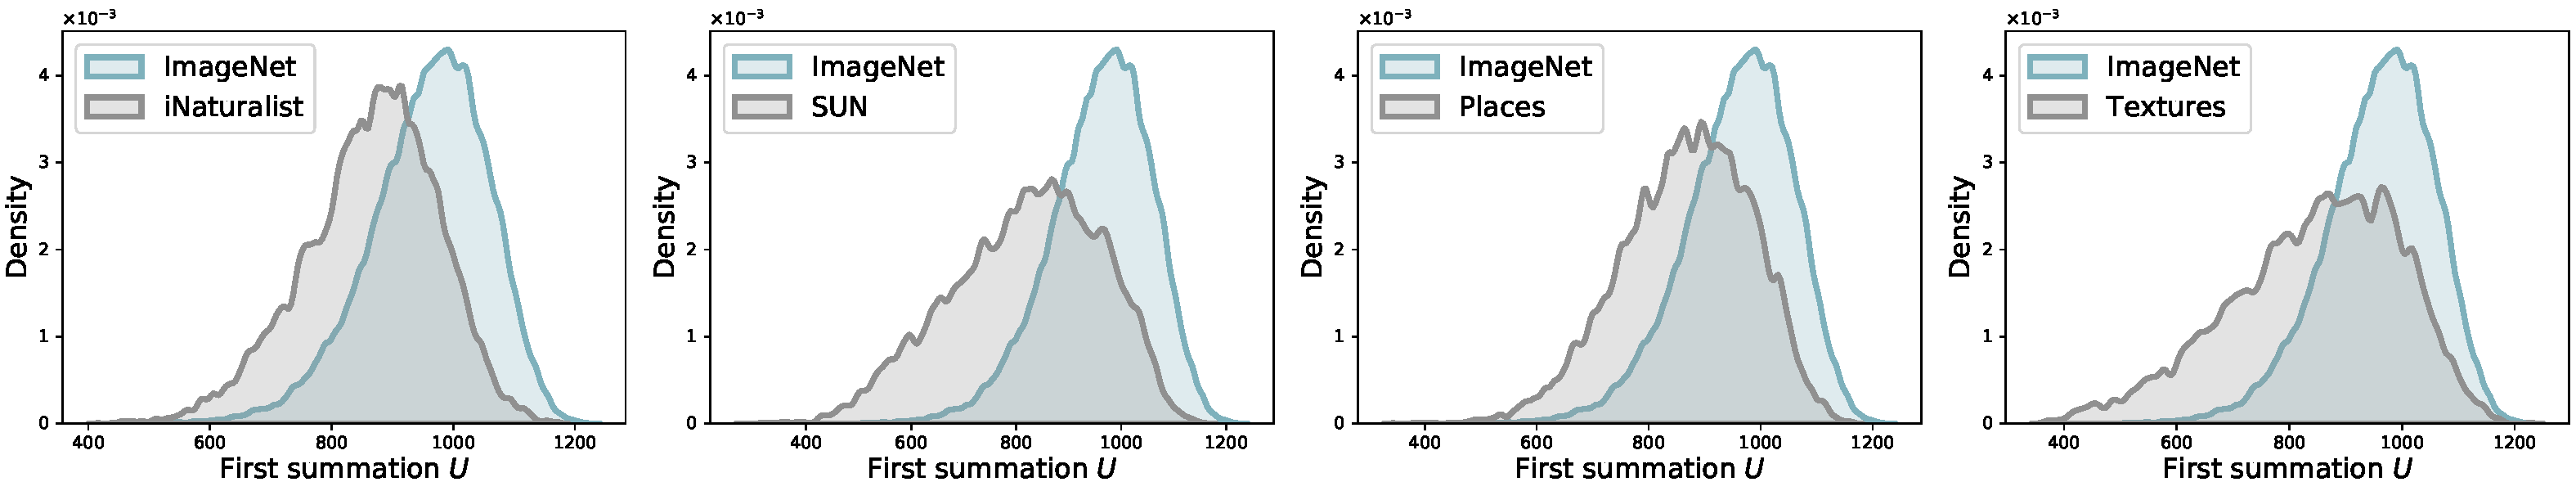
\includegraphics[width=1.0\textwidth]{figures/first_summation_final.pdf}
    \caption{Distribution of  $U$}
    \end{subfigure}
    % \vspace{1cm}
    \begin{subfigure}{1\textwidth}
    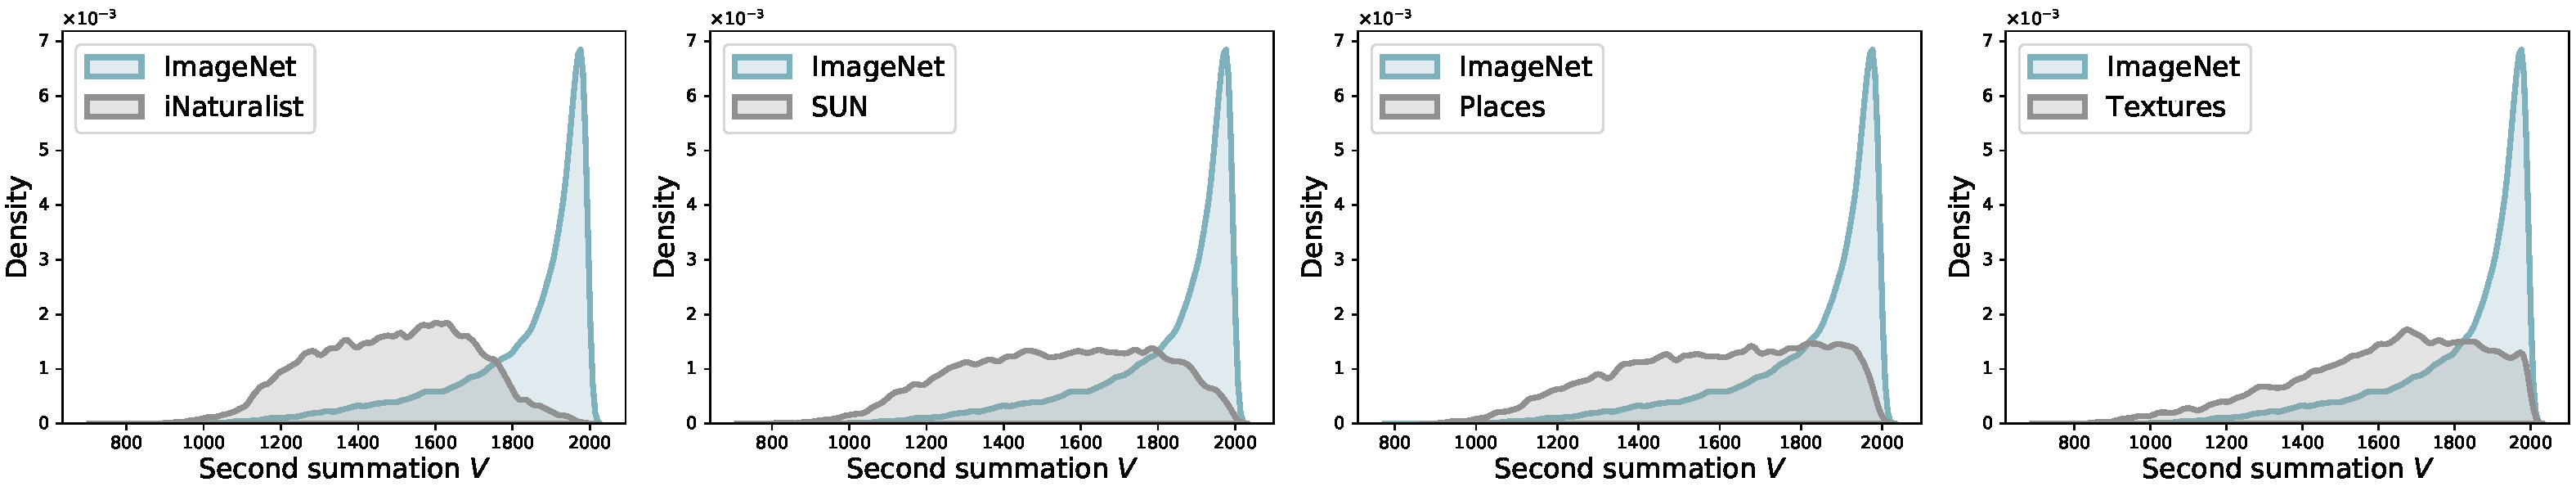
\includegraphics[width=1.0\textwidth]{figures/second_summation_final.pdf}
    \caption{Distribution of $V$}
    \end{subfigure}
    \caption{\small{We show the distributions of the two summations decomposed from the $L_1$-norm of the last layer gradient, for both in-distribution data (blue) and out-of-distribution data (gray). }}
    \label{fig:first_and_second_sum}
    %\vspace{-0.4cm}
\end{figure*}

%\vspace{-0.1cm}
\textbf{{GradNorm} captures joint information between feature and output} First we can rewrite the KL divergence between the softmax prediction and the uniform target as:
% \begin{equation*}
%     \begin{split}
%         D_\text{KL} (\*u \lVert \text{softmax}(f(\*x))) &= - \frac{1}{C}\sum_{c=1}^C \log{ \frac{e^{{f_c} / T}}{\sum_{j=1}^C e^{{f_{j}} / T}}} \\
%         & = - \frac{1}{C} \left( \frac{1}{T}\sum_{c=1}^C f_c - C \cdot \log{{\sum_{j=1}^C e^{{f_{j}} / T}}} \right).
%     \end{split}
% \end{equation*}
\begin{align*}
        D_\text{KL} (\*u \lVert \text{softmax}(f(\*x))) & = - \frac{1}{C}\sum_{c=1}^C \log{ \frac{e^{{f_c} / T}}{\sum_{j=1}^C e^{{f_{j}} / T}}} - H(\*u)  \\&= - \frac{1}{C} \left( \frac{1}{T}\sum_{c=1}^C f_c - C \cdot \log{{\sum_{j=1}^C e^{{f_{j}} / T}}} \right) - H(\*u).
\end{align*}

Then we consider the derivative of $D_\text{KL}$ \wrt each output logit $f_c$:
% \begin{equation*}
%     \begin{split}
%         \frac{\partial D_\text{KL}}{\partial f_c}
%         &= -\frac{1}{CT} \left( 1 + CT \cdot \frac{\partial \left( \log{{\sum_{j=1}^C e^{{f_{j}} / T}}}\right)}{\partial f_c} \right) \\
%         &= -\frac{1}{CT} \left( 1 - C \cdot \frac{e^{f_c / T}}{\sum_{j=1}^C e^{{f_{j}} / T}} \right).
%     \end{split}
% \end{equation*}
\begin{align*}
        \frac{\partial D_\text{KL}}{\partial f_c}
       & = -\frac{1}{CT} \left( 1 - CT \cdot \frac{\partial \left( \log{{\sum_{j=1}^C e^{{f_{j}} / T}}}\right)}{\partial f_c} \right) \\
    &    = -\frac{1}{CT} \left( 1 - C \cdot \frac{e^{f_c / T}}{\sum_{j=1}^C e^{{f_{j}} / T}} \right).
\end{align*}

Next the derivative of $ D_\text{KL}$ \wrt the weight matrix can be written as:
% \begin{equation*}
%     \begin{split}
%         \frac{\partial  D_\text{KL}}{\partial \mathbf{W}} =& \mathbf{x} \frac{\partial  D_\text{KL}}{\partial f} 
%         = -\frac{1}{CT} \cdot [x_1, x_2, \dots, x_m]^{\top}\\
%         &[1 - C \cdot \frac{e^{f_1 / T}}{\sum_{j=1}^C e^{{f_{j}} / T}}, \dots, 1 - C \cdot \frac{e^{f_C / T}}{\sum_{j=1}^C e^{{f_{j}} / T}}].
%     \end{split}
% \end{equation*}
\begin{equation*}
        \frac{\partial  D_\text{KL}}{\partial \mathbf{W}} = \mathbf{x} \frac{\partial  D_\text{KL}}{\partial f} 
        = -\frac{1}{CT} \cdot [x_1, x_2, \dots, x_m]^{\top}
        [1 - C \cdot \frac{e^{f_1 / T}}{\sum_{j=1}^C e^{{f_{j}} / T}}, \dots, 1 - C \cdot \frac{e^{f_C / T}}{\sum_{j=1}^C e^{{f_{j}} / T}}].
\end{equation*}

Finally, the $L_1$-norm of gradients of the weight matrix is simply the sum of absolute values of all elements in the gradient matrix:
\begin{equation}
    \begin{split}
        S(\*x) &= \sum_{i=1}^m \sum_{j=1}^C \left|\left(\frac{\partial  D_\text{KL}}{\partial \mathbf{W}}\right)_{ij}\right| = \frac{1}{CT} \sum_{i=1}^m \left( |x_i| \left(\sum_{j=1}^C \left|1 - C \cdot \frac{e^{f_j / T}}{\sum_{j=1}^C e^{{f_{j}} / T}}\right|\right)\right) \\
        &= \frac{1}{CT}  \left(\sum_{i=1}^m |x_i|\right) \left(\sum_{j=1}^C \left|1 - C \cdot \frac{e^{f_j / T}}{\sum_{j=1}^C e^{{f_{j}} / T}}\right|\right) \\
        & \triangleq \frac{1}{CT} U \cdot V,
    \end{split}
    \label{eq:decomp}
\end{equation}
where the first multiplicative term $U=\sum_{i=1}^m |x_i|$ is the $L_1$-norm of the feature vector $\*x$, and the second term $V$ characterizes information in the output space. 


%\vspace{-0.3cm}
\textbf{Ablation on $U$ and $V$} In Figure~\ref{fig:first_and_second_sum} we plot distribution densities of $U$ and $V$, for both ID and OOD data. %We observe that the second term $V$ in the decomposed gradient plays a crucial role in distinguishing between in- and out-of-distribution samples. 
It is important to note that $U$ and $V$ measure statistical distributions in the feature space and the output space, respectively. Therefore, \texttt{GradNorm} captures the joint information between the feature and the output space. The multiplication of both $U$ and $V$ results in an overall stronger separability between ID and OOD, as seen in Figure~\ref{subfig:score_dist_uniform}. We report the OOD detection performance using $U$ and $V$ individually as scoring functions in Table~\ref{tab:uv_ood_performance}, both of which are less competitive than \texttt{GradNorm}.

\begin{table}[h]
    \centering
\scriptsize{
\begin{tabular}{c|C{0.04\textwidth}C{0.05\textwidth}|C{0.04\textwidth}C{0.05\textwidth}|C{0.04\textwidth}C{0.05\textwidth}|C{0.04\textwidth}C{0.05\textwidth}|C{0.04\textwidth}C{0.05\textwidth}}
\toprule
 \multicolumn{1}{c|}{\multirow{3}{*}{\textbf{Method}}} & \multicolumn{2}{c|}{\textbf{iNaturalist}}    & \multicolumn{2}{c|}{\textbf{SUN}}            & \multicolumn{2}{c|}{\textbf{Places}}         & \multicolumn{2}{c|}{\textbf{Textures}}       & \multicolumn{2}{c}{\textbf{Average}}        \\ 
\cline{2-11} 
                                                                                  \multicolumn{1}{c|}{}                                 & \scriptsize{FPR95}                & \scriptsize{AUROC}                 & \scriptsize{FPR95}                & \scriptsize{AUROC}              & \tiny{FPR95}                & \scriptsize{AUROC}                 & \scriptsize{FPR95}                & \scriptsize{AUROC}                 & \scriptsize{FPR95}                & \scriptsize{AUROC}               \\
                                                                                      \multicolumn{1}{c|}{}                                 & \multicolumn{1}{c}{$\downarrow$} & \multicolumn{1}{c|}{$\uparrow$} & \multicolumn{1}{c}{$\downarrow$} & \multicolumn{1}{c|}{$\uparrow$} & \multicolumn{1}{c}{$\downarrow$} & \multicolumn{1}{c|}{$\uparrow$} & \multicolumn{1}{c}{$\downarrow$} & \multicolumn{1}{c|}{$\uparrow$} & \multicolumn{1}{c}{$\downarrow$} & \multicolumn{1}{c}{$\uparrow$}  \\ \midrule
                                                                                      %KL (output space) & 64.91 & 88.48 & 65.33 & 85.32 & 73.02 & 81.37 & 80.87 & 75.79 & 71.03 & 82.74 \\ \midrule
                                                                                    U (feature space) &  77.84 & 74.33 & 61.90 & 78.74 & 76.42 & 72.75 & 67.84 & 72.77 & 71.00 & 74.65\\
                                                                                    V (output space) & 66.14 & 88.45 & 69.49 & 83.13 & 75.95 & 78.98 & 81.13 & 76.06 & 73.18 & 81.66  \\
                                                                                   \textbf{ U $\cdot$ V (Joint space)} & \textbf{50.05} & \textbf{90.33} & \textbf{46.48} & \textbf{89.03} & \textbf{60.86} & \textbf{84.82} & \textbf{61.42} & \textbf{81.07} & \textbf{54.70} & \textbf{86.31} \\
                                                            
\bottomrule
\end{tabular}
}
    \caption{\small{OOD detection performance using the decomposed $U$ (feature space) and $V$ (output space) as scoring functions. Model is ResNetv2-101 trained on ImageNet-1k~\cite{deng2009imagenet}.}}
    \label{tab:uv_ood_performance}
    \vspace{-0.5cm}
\end{table}

%We also compare with the performance of directly using the KL divergence derived from Equation~\ref{eq:kl} as OOD scoring function. Interestingly, even though both the feature space metric ($U$) and the output space metric ($V$) under-performs KL divergence, $U \cdot V$ yields significantly better performance than the KL divergence extracted from the output space, demonstrating the superiority of combining information from both output space and feature space for OOD detection.



%\SL{point out that the decomposition captures both feature and output}



% The overlapping between in- and out-of-distribution data is significantly smaller in the distribution of $V$ than that in the distribution of $U$. Therefore, we can reach a conclusion that the second summation $V$ in the decomposed gradient plays a crucial role in distinguishing between in- and out-of-distribution samples.


% \section{Discussion}
% \label{sec:discussion}
% In this section, we discuss connections and differences between \texttt{GradNorm} with previous OOD detection approaches that utilize gradient information, in particular ODIN (Section~\ref{sec:connection_with_odin}) and \citeauthor{lee2020gradients}'s approach (Section~\ref{sec:connection_with_al}). %and Energy Score (Section~\ref{sec:connection_with_energy}). Then we will provide mathematical and visual interpretations of the best variants of our method, $L_1$-norm of the last layer gradients, in Section~\ref{sec:decomposition}.
% %that utilize the information obtained from gradient space to perform out-of-distribution (OOD) detection. In Section 6.1 we will discuss the methodology introduced in ODIN \cite{hsu2020} and in Section 6.2 will discuss the methodology introduced by AlRegib \& Lee \cite{lee2020gradients}.


% \subsection{Comparison with ODIN}
% \label{sec:connection_with_odin}
% \citeauthor{liang2018enhancing} proposed a framework for OOD detection which utilizes small perturbations obtained from input gradients for input pre-processing. Perturbation in ODIN is inspired by the adversarial perturbations introduced in \cite{goodfellow2014explaining}. The goal of ODIN perturbations is to increase the softmax score of any given input by reinforcing the model's belief on the predicted label. Ultimately the perturbations have been found to create a greater gap between the softmax scores of ID and OOD inputs, thus making them more separable and improving the performance of OOD detection.

% Despite effectiveness, it is important to note that ODIN only uses gradients \emph{implicitly} through input perturbation, and OOD scores are still derived from the output space of the perturbed inputs. Different from ODIN, \texttt{GradNorm} utilizes information solely obtained from the {gradient space}. The effectiveness of \texttt{GradNorm} beckons a revisiting of combining information obtainable from the gradient space and the output space, which could provide a stronger method. We leave this question open for future exploration.

% \vspace{-0.1cm}
% \subsection{Comparison with \citeauthor{lee2020gradients}}
% \label{sec:connection_with_al}
% \citeauthor{lee2020gradients} proposed an OOD detection framework using the $L_2$-norm of gradients. Importantly, they do not directly use gradient norms for OOD detection, but instead, use them as the basis for training an additional binary classifier for detection. Furthermore, the binary classifier is trained on the OOD datasets, which can unfairly overfit to the test data and does not suit OOD-agnostic settings in the real world. In contrast, our methodology mitigates the shortcomings in that \texttt{GradNorm} (1) does not require any new model training, (2) is hyperparameter-free, and (3) is suitable for OOD-agnostic settings. In fact, our experiments suggest that the performance of \citeauthor{lee2020gradients}'s method is very limited when no prior knowledge about OOD data is available. As shown in Table~\ref{table:main}, \texttt{GradNorm} reduces the FPR95 by \textbf{15.45}\%.% in a fair comparison where no OOD data can be used in training for both methods.
% %\footnote{For \citeauthor{lee2020gradients}'s method, we use the gradients of uniform noise as a surrogate of OOD data to train the binary classifier.}.

% Additionally, our work comprehensively investigates and explains various important design choices in using gradient-based methods, which is otherwise missing in \citeauthor{lee2020gradients}. Furthermore, different from \citeauthor{lee2020gradients}, our evaluation is based on high-resolution large-scale datasets, which makes our results more relevant for the real world.

% \subsection{Connection with Energy Score}
% \label{sec:connection_with_energy}
% Our fully categorical cross-entropy loss has an intrinsic connection with the energy score which is a competitive method widely used in OOD detection~\cite{}. By definition, we can write the fully categorical cross-entropy loss as:
% \begin{equation*}
% \begin{split}
%   \mathcal{L} &= - \sum_{c=1}^C \log{ \frac{e^{{f_c} / T}}{\sum_{c'=1}^C e^{{f_{c'}} / T}}} \\
%   & = - \left( \frac{1}{T}\sum_{c=1}^C f_c - C \cdot \log{{\sum_{c'=1}^C e^{{f_{c'}} / T}}} \right),
% \end{split}
% \end{equation*}

% According to \citeauthor{}, the energy score is defined as:
% \begin{equation*}
%     E = -T \cdot \log{{\sum_{c'=1}^C e^{{f_{c'}} / T}}}
% \end{equation*}

% Therefore, our fully categorical cross-entropy loss can be written as:
% \begin{equation}
%   \mathcal{L} = - \frac{1}{T} \left(\sum_{c=1}^C f_c + C \cdot E \right),
% \end{equation}

%Thus we have built a connection between our fully categorical cross-entropy loss and the energy score, serving as another interpretation of why our method works well.

\vspace{-0.2cm}
\section{Discussion}
\label{sec:discussion}
\vspace{-0.2cm}
To the best of our knowledge, there is very limited prior work studying how to use gradients for OOD detection.  In this section, we discuss connections and differences between \texttt{GradNorm} and previous OOD detection approaches that utilize gradient information, in particular ODIN (Section~\ref{sec:connection_with_odin}) and \citeauthor{lee2020gradients}'s approach (Section~\ref{sec:connection_with_al}).

%and Energy Score (Section~\ref{sec:connection_with_energy}). Then we will provide mathematical and visual interpretations of the best variants of our method, $L_1$-norm of the last layer gradients, in Section~\ref{sec:decomposition}.
%that utilize the information obtained from gradient space to perform out-of-distribution (OOD) detection. In Section 6.1 we will discuss the methodology introduced in ODIN \cite{hsu2020} and in Section 6.2 will discuss the methodology introduced by AlRegib \& Lee \cite{lee2020gradients}.

\vspace{-0.2cm}
\subsection{Comparison with ODIN}
\label{sec:connection_with_odin}
\vspace{-0.1cm}

Our work is inspired by ODIN~\cite{liang2018enhancing}, which first explored using gradient information for OOD detection. In particular, ODIN proposed using input pre-processing by adding small perturbations obtained from the input gradients. The goal of ODIN perturbations is to increase the softmax score of any given input by reinforcing the model's belief in the predicted label. Ultimately the perturbations have been found to create a greater gap between the softmax scores of ID and OOD inputs, thus making them more separable and improving the performance of OOD detection.

It is important to note that ODIN only uses gradients \emph{implicitly} through input perturbation, and OOD scores are still derived from the output space of the perturbed inputs. Different from ODIN, \texttt{GradNorm} utilizes information solely obtained from the {gradient space}. The effectiveness of \texttt{GradNorm} beckons a revisiting of combining information obtainable from the gradient space and the output space, which could provide a stronger method. We leave this question for future exploration.

\vspace{-0.2cm}
\subsection{Comparison with \citeauthor{lee2020gradients}}
\label{sec:connection_with_al}
\vspace{-0.1cm}
\citeauthor{lee2020gradients}~\cite{lee2020gradients} proposed to train an auxiliary binary classifier using gradient information from ID and OOD data. Importantly, they do not directly use gradient norms for OOD detection, but instead, use them as the input for training a separate binary classifier. Furthermore, the binary classifier is trained on the OOD datasets, which can unfairly overfit the test data and does not suit OOD-agnostic settings in the real world. In contrast, our methodology mitigates the shortcomings in that \texttt{GradNorm} (1) does not require any new model training, (2) is hyperparameter-free, and (3) is suitable for OOD-agnostic settings. For these reasons, these two methods are not directly comparable. However, for completeness, we also reproduce \citeauthor{lee2020gradients}'s method using random noise as a surrogate of OOD data and compare it with \texttt{GradNorm} in Appendix~\ref{app:comparison_with_la}. \texttt{GradNorm} outperforms their approach by 15.45\% in FPR95 in this fair comparison.

Moreover, we provide comprehensive ablation studies and analyses on different design choices in using gradient-based methods for OOD detection (network architectures, gradients at different layers, loss functions for backpropagation, different $L_p$-norms, diverse evaluation datasets, and different temperatures, etc.), which were previously not studied in~\cite{lee2020gradients}. In particular, \citeauthor{lee2020gradients} utilize $L_2$-norm gradients without comparing them with other norms. Our ablation study leads to the new finding that $L_1$-norm works best among all variants with \texttt{GradNorm}, and outperforms $L_2$-norm by up to 22.31\% in FPR95. Furthermore, \citeauthor{lee2020gradients} utilize gradients from all layers to train a separate binary classifier, which can cause the computational cost to become intractable for deeper and larger models. In contrast, with \texttt{GradNorm} we show that the last layer gradient will always yield the best performance among all gradient set selections. Consequently, \texttt{GradNorm} incurs negligible computational cost. We believe such thorough understandings will be valuable for the field.


\vspace{-0.1cm}
\section{Related Work}
\label{sec:related_work}
\vspace{-0.3cm}
% \textbf{Discriminative-based OOD detection} \citeauthor{hendrycks2016baseline}~\cite{hendrycks2016baseline} proposed a baseline approach for OOD detection utilizing the maximum softmax probability from a pre-trained model. Several works attempt to improve the OOD detection performance by calibrating confidence scores~\cite{liang2018enhancing, hsu2020generalized} or energy score~\cite{liu2020energy} derived from the output space. Information from the feature space~\cite{lee2018simple} was proven effective on small-scale benchmarks. Other methods seek improvements using deep ensembles~\cite{lakshminarayanan2017simple} or adding a special branch for confidence estimation~\cite{devries2018learning}. These approaches derive OOD score either from output or feature space. In contrast, we show that \emph{gradient space} carries surprisingly useful information for OOD detection, which was underexplored in the literature.



\paragraph{OOD uncertainty estimation with discriminative models}  The problem of classification with rejection can date back to early works on abstention~\cite{chow1970optimum, fumera2002support}, which considered simple model families such as SVMs~\cite{cortes1995support}.
The phenomenon of neural networks' overconfidence in out-of-distribution data is first revealed by \citeauthor{nguyen2015deep}~\cite{nguyen2015deep}.
Early works attempted to improve the OOD uncertainty estimation by proposing the ODIN score~\citep{hsu2020generalized, liang2018enhancing} and Mahalanobis
distance-based confidence score~\citep{lee2018simple}.
Recent work by \citeauthor{liu2020energy}~\citep{liu2020energy} proposed using an energy score for OOD uncertainty estimation, which can be easily derived from a discriminative classifier and demonstrated advantages over the softmax confidence score both empirically and theoretically. ~\citeauthor{wang2021canmulti}~\cite{wang2021canmulti} further showed an energy-based approach  can improve OOD uncertainty estimation for multi-label classification networks. \citeauthor{huang2021mos}~\cite{huang2021mos} revealed that approaches developed for common CIFAR benchmarks might not translate effectively into a large-scale ImageNet benchmark, highlighting the need to evaluate OOD uncertainty estimation in a large-scale real-world setting.  %proposed a group-based OOD detection method that scales effectively to large-scale ImageNet benchmark. %\citeauthor{lin2021mood}~\cite{lin2021mood} proposed the first dynamic OOD inference framework that improved
%the computational efficiency of OOD detection. 
Existing approaches derive OOD scores from either output or feature space. In contrast, we show that \emph{gradient space} carries surprisingly useful information for OOD uncertainty estimation, which was underexplored in the literature.

% \paragraph{Distributional shifts} Literature in OOD detection is commonly concerned about model reliability and detection of label-space shifts where the OOD inputs have disjoint labels and therefore \emph{should not be predicted by the model}.  While other works have considered domain shifts~\citep{hsu2020generalized} or covariate shifts~\citep{ovadia2019can}, they are more relevant for evaluating domain generalization and robustness performance---in which case the goal is to make the model classify accurately into the existing classes. \texttt{GradNorm} is especially designed to detect label-space shifts rather than covariate shifts, and we caution the community to differentiate the two problems of detection vs. generalization, as well as the evaluation protocols.

% Covariate-shifted data is expected to have a higher GradNorm because the predictions can concentrate on the ground truth class (if the model indeed can generalize well). For example, we have verified this on pairs (e.g., CIFAR-10  vs. CIFAR-10C) and observed that the GradNorm distribution of CIFAR-10C is similar to that of CIFAR-10. We caution the community to differentiate the two problems of detection vs. generalization, as well as the evaluation protocols. %We emphasize that semantic label shift is more akin to OOD detection task, which concerns model reliability and detection of shifts where the inputs have disjoint labels from ID data and therefore \emph{should not be predicted by the model}.
 
% However, this method can unfairly overfit the OOD test datasets and does not suit OOD-agnostic settings in the real world. In contrast, \texttt{GradNorm} is convenient without requiring training a separate classifier, and is completely hyperparameter-free without the need for tuning on validation data. \citeauthor{lee2020gradients}~\cite{lee2020gradients} proposed an OOD detection framework using the $L_2$-norm of gradients. Importantly, they do not directly use gradient norms for OOD detection, but instead, use them as the input for training a separate binary classifier. Furthermore, the binary classifier is trained on the OOD datasets, which can unfairly overfit to the test data and does not suit OOD-agnostic settings in the real world. In contrast, our methodology mitigates the shortcomings in that \texttt{GradNorm} (1) does not require any new model training, (2) is hyperparameter-free, and (3) is suitable for OOD-agnostic settings. 

 
 
% \textbf{OOD detection with auxiliary outlier data} ~ An orthogonal line of work reveals that models can produce lower confidence on anomalous samples with exposure to auxiliary outlier data~\cite{bevandic2018discriminative,geifman2019selectivenet,malinin2018predictive,mohseni2020self,subramanya2017confidence}. Auxiliary outlier data can either be realistic images~\cite{hendrycks2018deep,liu2020energy, mohseni2020self,papadopoulos2019outlier} or synthetic images generated by GANs~\cite{lee2018training}.
% %Several loss functions have been designed to regularize model predictions of the auxiliary outlier data towards uniform distributions~\cite{hendrycks2018deep,lee2017training}, a pre-defined class for OOD data~\cite{chen2020robust-new}, or higher energies~\cite{liu2020energy}.
% However, in many applications, it can be prohibitive to construct an auxiliary outlier dataset since the in-distribution data has a much larger coverage of concepts (e.g., ImageNet). Importantly, our method does not assume the availability of any auxiliary data, and can be \emph{flexibly} and \emph{easily} used for pre-trained models.

\vspace{-0.2cm}
\paragraph{OOD uncertainty estimation with generative models} ~ Alternative approaches for detecting OOD inputs resort to generative models that directly estimate density~\cite{dinh2017density,huang2017stacked, kingma2014autoencoding, oord2016conditional, rezende2014stochastic,  tabak2013family}. An input is deemed as OOD if it lies in the low-likelihood regions. A plethora of literature has emerged to utilize generative models for OOD detection~\cite{ kirichenko2020normalizing, ren2019likelihood, schirrmeister2020understanding, serra2019input, wang2020further, winkens2020contrastive, xiao2020likelihood}.
%Additionally, \citeauthor{pope20a} shows that flow-based generative models are sensitive under adversarial attacks. 
%Several methods improve OOD detection with generative models, such as improved metrics~\cite{choi2018generative}, likelihood ratios~\cite{ren2019likelihood,serra2019input} and likelihood regret~\cite{xiao2020likelihood}.
Interestingly, \citeauthor{nalisnick2018deep}~\cite{nalisnick2018deep} showed that deep generative models can assign a high likelihood to OOD data.
Moreover, generative models can be prohibitively challenging to train and optimize, and the performance can often lag behind the discriminative counterpart. In contrast, our method relies on a discriminative classifier, which is easier to optimize and achieves stronger performance. %Therefore, we primarily focus on discriminative-model-based OOD methods in this work.

%Once again, many of these approaches differentiates itself significantly from our methodology as we primarily focus on showcasing the informativeness of the gradient space for OOD detection.

% \textbf{Gradient-based OOD detection} ~ Several works take pioneering steps in exploring gradient information in OOD detection~\cite{liang2018enhancing, lee2020gradients}. ODIN utilizes input gradients to generate a small perturbation to the original image, which will in turn improve the distinguishability between ID and OOD data~\cite{liang2018enhancing}. \citeauthor{lee2020gradients} propose to train a new binary classifier with extracted gradients from both ID and OOD data as input, which can be infeasible with the absence of auxiliary outlier data. These works inspire our work by demonstrating the effectiveness of gradients in context of OOD detection. However, they have limited effectiveness and feasibility compared with \texttt{GradNorm}. An in-depth discussion of these methods are presented in Section~\ref{sec:discussion}.


%\SL{highlight why auxiliary data and generative modeling is infeasible in large-scale setting.}
\vspace{-0.2cm}
\paragraph{Distributional shifts} Distributional shifts have attracted increasing research interests. It is important to recognize and differentiate various types of distributional shift problems. Literature in OOD detection is commonly concerned about model reliability and detection of label-space shifts~\cite{hendrycks2016baseline, liang2018enhancing, liu2020energy}, where the OOD inputs have disjoint labels \wrt ID data and therefore \emph{should not be predicted by the model}. Meanwhile, some works considered covariate shifts in the input space~\citep{hendrycks2019benchmarking, malinin2021shifts, ovadia2019can}, where inputs can be corruption-shifted or domain-shifted~\citep{hsu2020generalized}. However, covariate shifts are commonly used to evaluate model robustness and domain generalization performance, where the label space $\mathcal{Y}$ remains the same during test time. It is important to note that our work focuses on the detection of shifts where the model should not make any prediction, instead of covariate shifts where the model is expected to \emph{generalize}. %We caution the community to differentiate the two types of distributional shifts, which correspond to two drastically different problems, detection vs. generalization.

%(a.k.a. domain shifts~\cite{lakshminarayanan2017simple})

\vspace{-0.3cm}
\section{Conclusion}
\vspace{-0.2cm}
\label{sec:conclusion}
In this paper, we propose \texttt{GradNorm}, a novel OOD uncertainty estimation approach utilizing information extracted from the \emph{gradient space}. %, along with a novel loss function for gradient computation and several heuristic strategies for gradient selection. %Specifically, we utilize information provided through backpropagated gradients in relation to an binary cross entropy loss function to build the foundations of our OOD score. We showcase the effectiveness of the methodology in a large input space setting, achieving % TODO Some numerical data here! 
%and present extensive ablations on our methodology. Additionally, we present a series of ablations showcasing some potential future research directions. 
Experimental results show that our gradient-based method can improve the performance of OOD detection by up to  {16.33}\% in FPR95, establishing superior performance.
Extensive ablations provide further understandings of our approach. 
We hope that our research brings to light the informativeness of gradient space, and inspires future work to utilize gradient space for OOD uncertainty estimation.


\vspace{-0.2cm}
\section{Societal Impact}
\label{sec:broad}
\vspace{-0.3cm}
Our project aims to improve the reliability and safety of modern machine learning models.
This stands to benefit a wide range of fields and societal activities. We believe out-of-distribution uncertainty estimation is an increasingly critical component of systems that range from consumer and business applications (e.g., digital content understanding) to transportation (e.g., driver assistance systems and autonomous vehicles), and to health care (e.g., unseen disease identification). Many of these applications require classification models in operation.\@
Through this work and by releasing our code, we hope to provide machine learning researchers with a new methodological perspective and offer machine learning practitioners an easy-to-use tool that renders safety against OOD data in the real world. While we do not anticipate any negative consequences to our work, we hope to continue to build on our framework in future work. 
\vspace{-0.2cm}
\section*{Acknowledgement}
\vspace{-0.3cm}
 Research is supported by the Office of the Vice Chancellor for Research and Graduate Education (OVCRGE) with funding from the Wisconsin Alumni Research Foundation (WARF).

% Acknowledgements should only appear in the accepted version.
% \section*{Acknowledgements}
% \newpage

% Citing informative outlier mining paper as we used their codebase as a baseline 
% \nocite{chen2020}
\newpage
\bibliography{neurips_2021}
\bibliographystyle{plainnat}


%%%%%%%%%%%%%%%%%%%%%%%%%%%%%%%%%%%%%%%%%%%%%%%%%%%%%%%%%%%%
% \newpage
% \section*{Checklist}

% %%% BEGIN INSTRUCTIONS %%%
% % The checklist follows the references.  Please
% % read the checklist guidelines carefully for information on how to answer these
% % questions.  For each question, change the default \answerTODO{} to \answerYes{},
% % \answerNo{}, or \answerNA{}.  You are strongly encouraged to include a {\bf
% % justification to your answer}, either by referencing the appropriate section of
% % your paper or providing a brief inline description.  For example:
% % \begin{itemize}
% %   \item Did you include the license to the code and datasets? \answerYes{See Section~\ref{gen_inst}.}
% %   \item Did you include the license to the code and datasets? \answerNo{The code and the data are proprietary.}
% %   \item Did you include the license to the code and datasets? \answerNA{}
% % \end{itemize}
% % Please do not modify the questions and only use the provided macros for your
% % answers.  Note that the Checklist section does not count towards the page
% % limit.  In your paper, please delete this instructions block and only keep the
% % Checklist section heading above along with the questions/answers below.
% %%% END INSTRUCTIONS %%%

% \begin{enumerate}

% \item For all authors...
% \begin{enumerate}
%   \item Do the main claims made in the abstract and introduction accurately reflect the paper's contributions and scope?
%     \answerYes{See Sections~\ref{sec:experiments} and ~\ref{sec:analysis}}
%   \item Did you describe the limitations of your work?
%     \answerNA{}
%   \item Did you discuss any potential negative societal impacts of your work?
%     \answerNA{}
%   \item Have you read the ethics review guidelines and ensured that your paper conforms to them?
%     \answerYes{}
% \end{enumerate}

% \item If you are including theoretical results...
% \begin{enumerate}
%   \item Did you state the full set of assumptions of all theoretical results?
%     \answerYes{See Section~\ref{sec:analysis}}
% 	\item Did you include complete proofs of all theoretical results?
%     \answerYes{See Section~\ref{sec:analysis}}
% \end{enumerate}

% \item If you ran experiments...
% \begin{enumerate}
%   \item Did you include the code, data, and instructions needed to reproduce the main experimental results (either in the supplemental material or as a URL)?
%     \answerYes{}
%   \item Did you specify all the training details (e.g., data splits, hyperparameters, how they were chosen)?
%     \answerYes{See experimental setups in Section~\ref{sec:experiments} and also Appendix~\ref{app:exp_detail}.}
% 	\item Did you report error bars (e.g., with respect to the random seed after running experiments multiple times)?
%     \answerNA{}
% 	\item Did you include the total amount of compute and the type of resources used (e.g., type of GPUs, internal cluster, or cloud provider)?
%     \answerYes{}
% \end{enumerate}

% \item If you are using existing assets (e.g., code, data, models) or curating/releasing new assets...
% \begin{enumerate}
%   \item If your work uses existing assets, did you cite the creators?
%     \answerYes{See Section~\ref{sec:experiments} Datasets.}
%   \item Did you mention the license of the assets?
%     \answerNA{}
%   \item Did you include any new assets either in the supplemental material or as a URL?
%     \answerNo{}
%   \item Did you discuss whether and how consent was obtained from people whose data you're using/curating?
%     \answerNA{}
%   \item Did you discuss whether the data you are using/curating contains personally identifiable information or offensive content?
%     \answerNA{}
% \end{enumerate}

% \item If you used crowdsourcing or conducted research with human subjects...
% \begin{enumerate}
%   \item Did you include the full text of instructions given to participants and screenshots, if applicable?
%     \answerNA{}
%   \item Did you describe any potential participant risks, with links to Institutional Review Board (IRB) approvals, if applicable?
%     \answerNA{}
%   \item Did you include the estimated hourly wage paid to participants and the total amount spent on participant compensation?
%     \answerNA{}
% \end{enumerate}

% \end{enumerate}

%%%%%%%%%%%%%%%%%%%%%%%%%%%%%%%%%%%%%%%%%%%%%%%%%%%%%%%%%%%%

% This document was modified from the file originally made available by
% Pat Langley and Andrea Danyluk for ICML-2K. This version was created
% by Iain Murray in 2018, and modified by Alexandre Bouchard in
% 2019 and 2021. Previous contributors include Dan Roy, Lise Getoor and Tobias
% Scheffer, which was slightly modified from the 2010 version by
% Thorsten Joachims & Johannes Fuernkranz, slightly modified from the
% 2009 version by Kiri Wagstaff and Sam Roweis's 2008 version, which is
% slightly modified from Prasad Tadepalli's 2007 version which is a
% lightly changed version of the previous year's version by Andrew
% Moore, which was in turn edited from those of Kristian Kersting and
% Codrina Lauth. Alex Smola contributed to the algorithmic style files.

\newpage
\appendix
\onecolumn
  
\begin{center}
    \Large{\textbf{Supplementary Material}}
\end{center}

% \section{ Categories in OOD Datasets}


% \label{app:ood_class}
% % To evaluate our approach, we consider a diverse collection of OOD test datasets, spanning various domains. We carefully curate the OOD evaluation benchmarks to make sure  concepts  in  these  datasets  are  not  overlapping  with ImageNet-1k~\cite{deng2009imagenet}. Below we provide the list of concepts chosen for each OOD dataset, including iNaturalist~\cite{van2018inaturalist}, SUN~\cite{xiao2010sun}, and Places365~\cite{zhou2017places}. We hope the information would allow future research to reproduce our results.
% % Below are the lists of categories chosen in each curated OOD dataset:

% \vspace{-0.4cm}
% \paragraph{iNaturalist} \textit{Coprosma lucida}, \textit{Cucurbita foetidissima}, \textit{Mitella diphylla}, \textit{Selaginella bigelovii}, \textit{Toxicodendron vernix}, \textit{Rumex obtusifolius}, \textit{Ceratophyllum demersum}, \textit{Streptopus amplexifolius}, \textit{Portulaca oleracea}, \textit{Cynodon dactylon}, \textit{Agave lechuguilla}, \textit{Pennantia corymbosa}, \textit{Sapindus saponaria}, \textit{Prunus serotina}, \textit{Chondracanthus exasperatus}, \textit{Sambucus racemosa}, \textit{Polypodium vulgare}, \textit{Rhus integrifolia}, \textit{Woodwardia areolata}, \textit{Epifagus virginiana}, \textit{Rubus idaeus}, \textit{Croton setiger}, \textit{Mammillaria dioica}, \textit{Opuntia littoralis}, \textit{Cercis canadensis}, \textit{Psidium guajava}, \textit{Asclepias exaltata}, \textit{Linaria purpurea}, \textit{Ferocactus wislizeni}, \textit{Briza minor}, \textit{Arbutus menziesii}, \textit{Corylus americana}, \textit{Pleopeltis polypodioides}, \textit{Myoporum laetum}, \textit{Persea americana}, \textit{Avena fatua}, \textit{Blechnum discolor}, \textit{Physocarpus capitatus}, \textit{Ungnadia speciosa}, \textit{Cercocarpus betuloides}, \textit{Arisaema dracontium}, \textit{Juniperus californica}, \textit{Euphorbia prostrata}, \textit{Leptopteris hymenophylloides}, \textit{Arum italicum}, \textit{Raphanus sativus}, \textit{Myrsine australis}, \textit{Lupinus stiversii}, \textit{Pinus echinata}, \textit{Geum macrophyllum}, \textit{Ripogonum scandens}, \textit{Echinocereus triglochidiatus}, \textit{Cupressus macrocarpa}, \textit{Ulmus crassifolia}, \textit{Phormium tenax}, \textit{Aptenia cordifolia}, \textit{Osmunda claytoniana}, \textit{Datura wrightii}, \textit{Solanum rostratum}, \textit{Viola adunca}, \textit{Toxicodendron diversilobum}, \textit{Viola sororia}, \textit{Uropappus lindleyi}, \textit{Veronica chamaedrys}, \textit{Adenocaulon bicolor}, \textit{Clintonia uniflora}, \textit{Cirsium scariosum}, \textit{Arum maculatum}, \textit{Taraxacum officinale officinale}, \textit{Orthilia secunda}, \textit{Eryngium yuccifolium}, \textit{Diodia virginiana}, \textit{Cuscuta gronovii}, \textit{Sisyrinchium montanum}, \textit{Lotus corniculatus}, \textit{Lamium purpureum}, \textit{Ranunculus repens}, \textit{Hirschfeldia incana}, \textit{Phlox divaricata laphamii}, \textit{Lilium martagon}, \textit{Clarkia purpurea}, \textit{Hibiscus moscheutos}, \textit{Polanisia dodecandra}, \textit{Fallugia paradoxa}, \textit{Oenothera rosea}, \textit{Proboscidea louisianica}, \textit{Packera glabella}, \textit{Impatiens parviflora}, \textit{Glaucium flavum}, \textit{Cirsium andersonii}, \textit{Heliopsis helianthoides}, \textit{Hesperis matronalis}, \textit{Callirhoe pedata}, \textit{Crocosmia × crocosmiiflora}, \textit{Calochortus albus}, \textit{Nuttallanthus canadensis}, \textit{Argemone albiflora}, \textit{Eriogonum fasciculatum}, \textit{Pyrrhopappus pauciflorus}, \textit{Zantedeschia aethiopica}, \textit{Melilotus officinalis}, \textit{Peritoma arborea}, \textit{Sisyrinchium bellum}, \textit{Lobelia siphilitica}, \textit{Sorghastrum nutans}, \textit{Typha domingensis}, \textit{Rubus laciniatus}, \textit{Dichelostemma congestum}, \textit{Chimaphila maculata}, \textit{Echinocactus texensis}

% \vspace{-0.4cm}

% \paragraph{SUN} \textit{badlands}, \textit{bamboo forest}, \textit{bayou}, \textit{botanical garden}, \textit{canal (natural)}, \textit{canal (urban)}, \textit{catacomb}, \textit{cavern (indoor)}, \textit{corn field}, \textit{creek}, \textit{crevasse}, \textit{desert (sand)}, \textit{desert (vegetation)}, \textit{field (cultivated)}, \textit{field (wild)}, \textit{fishpond}, \textit{forest (broadleaf)}, \textit{forest (needleleaf)}, \textit{forest path}, \textit{forest road}, \textit{hayfield}, \textit{ice floe}, \textit{ice shelf}, \textit{iceberg}, \textit{islet}, \textit{marsh}, \textit{ocean}, \textit{orchard}, \textit{pond}, \textit{rainforest}, \textit{rice paddy}, \textit{river}, \textit{rock arch}, \textit{sky}, \textit{snowfield}, \textit{swamp}, \textit{tree farm}, \textit{trench}, \textit{vineyard}, \textit{waterfall (block)}, \textit{waterfall (fan)}, \textit{waterfall (plunge)}, \textit{wave}, \textit{wheat field}, \textit{herb garden}, \textit{putting green}, \textit{ski slope}, \textit{topiary garden}, \textit{vegetable garden}, \textit{formal garden}

% \vspace{-0.4cm}

% \paragraph{Places} \textit{badlands}, \textit{bamboo forest}, \textit{canal (natural)}, \textit{canal (urban)}, \textit{corn field}, \textit{creek}, \textit{crevasse}, \textit{desert (sand)}, \textit{desert (vegetation)}, \textit{desert road}, \textit{field (cultivated)}, \textit{field (wild)}, \textit{field road}, \textit{forest (broadleaf)}, \textit{forest path}, \textit{forest road}, \textit{formal garden}, \textit{glacier}, \textit{grotto}, \textit{hayfield}, \textit{ice floe}, \textit{ice shelf}, \textit{iceberg}, \textit{igloo}, \textit{islet}, \textit{japanese garden}, \textit{lagoon}, \textit{lawn}, \textit{marsh}, \textit{ocean}, \textit{orchard}, \textit{pond}, \textit{rainforest}, \textit{rice paddy}, \textit{river}, \textit{rock arch}, \textit{ski slope}, \textit{sky}, \textit{snowfield}, \textit{swamp}, \textit{swimming hole}, \textit{topiary garden}, \textit{tree farm}, \textit{trench}, \textit{tundra}, \textit{underwater (ocean deep)}, \textit{vegetable garden}, \textit{waterfall}, \textit{wave}, \textit{wheat field}

% \begin{figure*}[h]
%     \centering
%     \includegraphics[width=0.9\textwidth]{figures/image_sample.pdf}
%     \caption{Samples of ID (green) and OOD images (orange)}
%     \label{fig:image_sample}
% \end{figure*}


% \begin{table*}[h]
%     \centering
% \begin{tabular}{l|c|cc}
% \toprule
% \multirow{2}{*}{\textbf{OOD data}}    & \multirow{2}{*}{\textbf{Norm Type}} & FPR95                & AUROC                \\
%                                       &                                     & \multicolumn{1}{c}{$\downarrow$} & \multicolumn{1}{c}{$\uparrow$} \\ \midrule
% \multirow{2}{*}{\textbf{iNaturalist}} & $L_1$-norm                             & 46.18                & 88.14                \\
%                                       & $L_2$-norm                             & 75.49                & 72.30                \\ \midrule
% \multirow{2}{*}{\textbf{SUN}}         & $L_1$-norm                             & 29.72                & 93.31                \\
%                                       & $L_2$-norm                             & 73.82                & 82.61                \\ \midrule
% \multirow{2}{*}{\textbf{Places}}      & $L_1$-norm                             & 45.18                & 88.19                \\
%                                       & $L_2$-norm                             & 87.90                & 74.00                \\ \midrule
% \multirow{2}{*}{\textbf{Textures}}    & $L_1$-norm                             & 16.59                & 96.12                \\
%                                       & $L_2$-norm                             & 43.39                & 84.16                \\ \midrule
% \multirow{2}{*}{\textbf{Average}}     & $L_1$-norm                             & 34.42                & 91.44                \\
%                                       & $L_2$-norm                             & 70.15                & 78.27                \\ \bottomrule
% \end{tabular}
%     \caption{OOD detection performance of \citeauthor{lee2020gradients}'s method under different norms.}
%     \label{tab:al_norm_ablation}
% \end{table*}

\section{Evaluation on CIFAR Benchmarks}
\label{app:cifar}
% \vspace{-0.3cm}
\textbf{Setup}
We additionally evaluate \texttt{GradNorm} on a common benchmark with CIFAR-10 and CIFAR-100~\cite{krizhevsky2009learning} as ID datasets, which is routinely used in literature~\cite{hendrycks2016baseline,liang2018enhancing,hsu2020generalized,liu2020energy,lee2018simple}. We use the standard split with 50,000 training images and 10,000 test images. We pre-train a ResNet-20~\cite{he2016deep} network for 100 epochs. The learning rate is initially 0.1, and decays by a factor of 10 at epochs 50, 75 and 90 respectively. We evaluate on four common OOD benchmark datasets: \texttt{SVHN}~\cite{netzer2011reading}, \texttt{LSUN} (crop)~\cite{yu2015lsun}, \texttt{Places365}~\cite{zhou2017places}, and \texttt{Textures}~\cite{cimpoi14describing}. 

\textbf{Results} %For comprehensive evaluation, we also report the performance of \texttt{GradNorm} v.s. all baselines on a small-scale benchmark with CIFAR-10/100~\cite{krizhevsky2009learning} as ID datasets, which is widely adopted in the prior literature. We train a ResNet-20~\cite{he2016deep} on CIFAR-10/100 datasets, and evaluate on 4 OOD datasets: SVHN~\cite{netzer2011reading}, LSUN (crop)~\cite{yu2015lsun}, Places365~\cite{zhou2017places}, and Textures~\cite{cimpoi14describing}. 
We summarize the results in Table~\ref{tab:cifar_results}, where \texttt{GradNorm} remains competitive. In particular, \texttt{GradNorm} reduces the average FPR95 by \textbf{8.77\%} on CIFAR-10 compared to the best baseline. On CIFAR-100, \texttt{GradNorm} outperforms the best baseline energy score~\cite{liu2020energy} by \textbf{14.47}\% in FPR95. Together with our large-scale evaluation in Section~\ref{sec:ablations}, \texttt{GradNorm} overall demonstrates superior performance compared to competitive methods in literature. While some baselines may require validation datasets, \texttt{GradNorm} is hyperparameter-free and can be used in OOD-agnostic setting. {Experimental details and hyperparameters of baseline methods can be found in Appendix~\ref{app:baseline}}. %\emph{Additional performance comparison with generative-based methods is provided in Appendix~\ref{sec:generative}}. 


\begin{table}[h]
    \centering
    \scriptsize{

\begin{tabular}{c|l|C{0.03\textwidth}C{0.045\textwidth}|C{0.03\textwidth}C{0.045\textwidth}|C{0.03\textwidth}C{0.045\textwidth}|C{0.03\textwidth}C{0.045\textwidth}|C{0.03\textwidth}C{0.045\textwidth}}
\toprule
\multirow{3}{*}{\textbf{ID Data}} & \multicolumn{1}{c|}{\multirow{3}{*}{\textbf{Method}}} & \multicolumn{2}{c|}{\textbf{SVHN}}           & \multicolumn{2}{c|}{\textbf{LSUN (crop)}}    & \multicolumn{2}{c|}{\textbf{Places365}}      & \multicolumn{2}{c|}{\textbf{Textures}}       & \multicolumn{2}{c}{\textbf{Average}}        \\ \cline{3-12} 
                                & \multicolumn{1}{c|}{}                                 & \tiny{FPR95}                & \tiny{AUROC}                 & \tiny{FPR95}                & \tiny{AUROC}              & \tiny{FPR95}                & \tiny{AUROC}                 & \tiny{FPR95}                & \tiny{AUROC}                 & \tiny{FPR95}                & \tiny{AUROC}               \\
                                                                                      & \multicolumn{1}{c|}{}                                 & \multicolumn{1}{c}{$\downarrow$} & \multicolumn{1}{c|}{$\uparrow$} & \multicolumn{1}{c}{$\downarrow$} & \multicolumn{1}{c|}{$\uparrow$} & \multicolumn{1}{c}{$\downarrow$} & \multicolumn{1}{c|}{$\uparrow$} & \multicolumn{1}{c}{$\downarrow$} & \multicolumn{1}{c|}{$\uparrow$} & \multicolumn{1}{c}{$\downarrow$} & \multicolumn{1}{c}{$\uparrow$}  \\ \midrule
\multirow{5}{*}{CIFAR-10}         & MSP\tiny{~\cite{hendrycks2016baseline}}                                                   & 66.09                & 89.86                 & 37.73                & 94.87                 & 70.05                & 85.99                 & 68.23                & 87.62                 & 60.53                & 89.59                \\
                                  & ODIN\tiny{~\cite{liang2018enhancing}}                                                  & 55.52                & 89.63                 & 2.32                 & 99.39                 & {45.86}       & {90.81}        & 52.78                & 89.99                 & 39.12                & 92.46                \\
                                %   & Generalized ODIN\tiny{~\cite{hsu2020generalized}}                                     & 34.71                & 90.49                 & 35.91                & 88.28                 & 77.11                & 72.83                 & 59.54                & 73.94                 & 51.82                & 81.39                \\
                                  & Energy\tiny{~\cite{liu2020energy}}                                                & 49.80                & 91.97                 & 3.86                 & 99.03                 & 46.48                & 90.55                 & 58.67                & 88.79                 & 39.70                & 92.59                \\
                                %   & Mahalanobis\tiny{~\cite{lee2018simple}}                                           & 60.00                & 80.92                 & 87.37                & 28.76                 & 90.19                & 57.63                 & 51.79                & 72.77                 & 72.34                & 60.02                \\
                                   & Mahalanobis\tiny{~\cite{lee2018simple}}                                           & 20.91 &	95.99 &	9.66 &	97.90 &	89.24 &	61.15 &	28.83 &	92.31 &	37.16 &	86.84              \\
                                %   & \citeauthor{lee2020gradients}\tiny{~\cite{lee2020gradients}}                                        & 76.09                & 60.98                 & 44.26                & 87.00                 & 72.11                & 72.04                 & 59.79                & 71.84                 & 63.06                & 72.96                \\
                                  & \textbf{GradNorm (ours)}                              & {17.76}       & {96.66}        & {0.23}        & {99.87}        & 57.85                & 85.20                 & {37.71}       & {90.76}        & \textbf{28.39}       & \textbf{93.12}       \\ 
                                  \midrule
\multirow{5}{*}{CIFAR-100}        & MSP\tiny{~\cite{hendrycks2016baseline}}                                                   & 86.33                & 72.56                 & 66.33                & 82.06                 & 87.57                & 69.05                 & 90.64                & 64.02                 & 82.72                & 71.92                \\
                                  & ODIN\tiny{~\cite{liang2018enhancing}}                                                  & 94.80                & 66.85                 & 26.14                & 95.09                 & 82.57                & 72.90                 & 89.91                & 66.35                 & 73.36                & 75.30                \\
                                %   & Generalized ODIN\tiny{~\cite{hsu2020generalized}}                                      & {66.48}       & {79.79}        & 90.89                & 55.33                 & 89.72                & 64.51                 & 94.52                & 55.52                 & 85.40                & 63.79                \\
                                  & Energy\tiny{~\cite{liu2020energy}}                                                & 89.03                & 76.42                 & 21.90                & 95.90                 & {82.55}       & {72.98}        & 88.81                & 66.74                 & 70.57                & 78.01                \\
                                %   & Mahalanobis\tiny{~\cite{lee2018simple}}                                           & 91.34                & 56.31                 & 48.40                & 84.46                 & 95.55                & 52.04                 & 63.88                & 67.10                 & 74.79                & 64.98                \\
                                  & Mahalanobis\tiny{~\cite{lee2018simple}}                                           & 81.46 &	81.71 &	68.97 &	90.74 &	96.50 &	50.35 &	42.71 &	87.48 &	72.41 &	77.57                \\
                                %   & \citeauthor{lee2020gradients}\tiny{~\cite{lee2020gradients}}                                       & 98.76                & 29.87                 & 97.07                & 43.98                 & 93.85                & 52.79                 & 77.25                & 58.43                 & 91.73                & 46.27                \\
                                  & \textbf{GradNorm (ours)}                              & 76.77                & 79.35                 & {1.12}        & {99.69}        & 88.74                & 65.99                 & {57.75}       & {81.83}        & \textbf{56.10}       & \textbf{81.72}       \\ 
\bottomrule
\end{tabular}
}
    \caption{\small{OOD detection performance on CIFAR-10 and CIFAR-100 benchmark. All methods utilize the standard ResNet-20~\cite{he2016deep} network.
}}
    \label{tab:cifar_results}
    \vspace{-0.5cm}
\end{table}

\section{Details of Experiments}
\label{app:exp_detail}

\subsection{Datasets}
\label{app:dataset}
\paragraph{Large-scale evaluation} We use ImageNet-1k~\cite{deng2009imagenet} as the in-distribution dataset, and evaluate on four OOD test datasets following the setup in \cite{huang2021mos}:
\begin{itemize}
    \item \textbf{iNaturalist}~\cite{van2018inaturalist} contains 859,000 plant and animal images across over 5,000 different species. Each image is resized to have a max dimension of 800 pixels. %We manually select 110 plant classes not present in ImageNet-1k, and randomly sample 10,000 images from these 110 classes. 
    We evaluate on 10,000 images randomly sampled from 110 classes that are disjoint from ImageNet-1k.
    \vspace{-0.1cm}
    \item \textbf{SUN}~\cite{xiao2010sun} contains over 130,000 images of scenes spanning 397 categories. SUN and ImageNet-1k have overlapping categories. %Therefore, we carefully select 50 nature-related concepts that are unique in SUN, such as \textit{forest} and \textit{iceberg}. We randomly sample 10,000 images from these 50 classes.
    We evaluate on 10,000 images randomly sampled from 50 classes that are disjoint from ImageNet labels.
    \vspace{-0.1cm}
    \item \textbf{Places}~\cite{zhou2017places} is another scene dataset with similar concept coverage as SUN. A chosen subset of 10,000 images across 50 classes (not contained in ImageNet-1k) are used.
    \vspace{-0.1cm}
    \item \textbf{Textures}~\cite{cimpoi14describing} contains 5,640 real-world texture images under 47 categories. We use the entire dataset for evaluation.
\end{itemize}

\paragraph{CIFAR benchmark} CIFAR-10 and CIFAR-100~\cite{krizhevsky2009learning} are widely used as ID datasets in the literature, which contain 10 and 100 classes, respectively. We use the standard split with 50,000 training images and 10,000 test images. We evaluate our approach on four common OOD datasets, which are listed below:
\begin{itemize}
    \item \textbf{SVHN}~\cite{netzer2011reading} contains color images of house numbers. There are ten classes of digits 0-9. We use the entire test set containing 26,032 images.
    \vspace{-0.1cm}
    \item \textbf{LSUN}~\cite{yu2015lsun} contains 10,000 testing images across 10 different scenes. Image patches of size 32$\times$32 are randomly cropped from this dataset.
    \vspace{-0.1cm}
    \item \textbf{Places365}~\cite{zhou2017places} contains large-scale photographs of scenes with 365 scene categories. There are 900 images per category in the test set. We randomly sample 10,000 images from the test set for evaluation.
    \vspace{-0.1cm}
    \item \textbf{Textures}~\cite{cimpoi14describing} contains 5,640 real-world texture images under 47 categories. We use the entire dataset for evaluation.
\end{itemize}

\subsection{Details of Baselines}
\label{app:baseline}

For the reader's convenience, we summarize in detail a few common techniques for defining OOD scores that measure the degree of ID-ness on the given sample.
%All the methods derive the score \emph{post hoc} on neural networks trained with in-distribution data only.
By convention, a higher (lower) score is indicative of being in-distribution (out-of-distribution).

% \paragraph{Softmax score} Hendrycks et al.~\cite{hendrycks2016baseline} the maximum softmax probability (MSP) to distinguish between $\Din$ and $\Dout$. In detail, suppose the label space is $\calY = \{1,\ldots,K\}$. We assume the classifier $f$ is defined in terms of a feature extractor $f : \calX \rightarrow \mathbb{R}^m$ and a linear multinomial regressor with weight matrix $W \in \mathbb{R}^{K \times m}$ and bias vector $\bb \in \mathbb{R}^K$. The prediction probability for each class is given by:
% \begin{equation}
%     P(y = k \mid \bx) = \softmax(W h(\bx) + \bb)_k.
% \end{equation}
% The softmax score is defined as $S_\mathrm{MSP}(\bx; f) := \max_k P(y = k \mid \bx)$.

% \textbf{ODIN score} Liang et al.~\cite{liang2018enhancing} introduced the ODIN score which  incorporates temperature scaling~\cite{hinton2015distilling,guo2017calibration} and adversarial perturbation~\cite{goodfellow2014explaining} to improve the separation of MSP for ID and OOD data.
% \begin{equation}
%     P(y = k \mid \mathbf{\tilde x}) = \softmax[ (W h(\mathbf{\tilde x}) + \bb)/T]_k,
% \end{equation}
% where $\mathbf{\tilde x}$ is the perturbed input. The ODIN score is defined as $S_\mathrm{ODIN}(\bx; f) := \max_k P(y = k \mid \mathbf{\tilde x})$.

% \textbf{Generalized ODIN} Hsu et al.~\cite{hsu2020generalized} extended ODIN by replacing the final fully connected layer to be the division of two functions $p$ and $q$. The predictive probability is given by:
% \begin{equation}
%     P(y = k \mid \mathbf{\tilde x}) = \softmax[ p(h(\mathbf{\tilde x})) /Tq(h(\mathbf{\tilde x}))]_k.
% \end{equation}
% where $q(h(\mathbf{\tilde x}))=\sigma\left(B N\left(\boldsymbol{w}_{q} h(\mathbf{\tilde x})+b_{q}\right)\right)$ and uses feature $h$ from the penultimate layer of
% neural networks sequentially through another linear layer, batch normalization (BN), and a sigmoid function $\sigma$. The $w_q$ and $b_q$ represent the learnable weights. And $p$ can be one of the following functions:
% \begin{equation} 
%     p^{I}(h(\mathbf{\tilde x})) &=\boldsymbol{w}_{i}^{\top} h(\mathbf{\tilde x}) +b_{i} \\ 
% \end{equation}
% \begin{equation}     
%     p^{E}(h(\mathbf{\tilde x})) &=-\left\|h(\mathbf{\tilde x}) -\boldsymbol{w}_{i}\right\|^{2} \\ 
% \end{equation}
% \begin{equation}    
%     p^{C}(h(\mathbf{\tilde x})) &=\frac{\boldsymbol{w}_{i}^{\top}  h(\mathbf{\tilde x}) }{\left\|\boldsymbol{w}_{i}\right\|\left\|h(\mathbf{\tilde x}) \right\|} 
% \end{equation}

% \paragraph{Energy score} The energy function~\cite{liu2020energy} maps the logit outputs to a scalar $S_\mathrm{Energy}(\bx; f) \in \mathbb{R}$, which is relatively lower for ID data:
% \begin{align}
% \label{eq:energy}
% S_\mathrm{Energy}(\bx; f)& =-\log \sum_{k=1}^{K}\exp(\*w_i^\top h(\bx) + b_i).
% \end{align}
% Note that Liu et al.~\cite{liu2020energy} used the \emph{negative energy score} for OOD detection, in order to align with the convention that $S(\*x;f)$ is higher for ID data and vice versa. 


% \paragraph{Mahalanobis distance} All the scores above operate on $K$-dimensional outputs of the multinomial regressor. 
% %As a result, discriminative information about ID vs. OOD data from the feature extractor $f$ may have been lost due to compression from the feature space $\mathbb{R}^m$. 
% In \cite{lee2018simple}, the authors instead  model the feature-level distribution as a mixture of class conditional Gaussians, and propose the \emph{Mahalanobis distance-based score}:
% \begin{equation}
%     S_\mathrm{Mahalanobis}(\bx; h) := \max_k - (h(\bx) - \hat{\mu}_k)^\top \hat{\Sigma} (h(\bx) - \hat{\mu}_k),
% \end{equation}
% where $\hat{\mu}_k$ is the estimated feature vector mean for class $k$ and $\hat{\Sigma}$ is the estimated covariance matrix (tied across classes). %This method can be extended to incorporate lower-level features from the network as well.



\textbf{MSP~\cite{hendrycks2016baseline}} propose to use the maximum softmax score to detect OOD samples.


\paragraph{ODIN~\cite{liang2018enhancing}} \citeauthor{liang2018enhancing} improved OOD detection with temperature scaling and input perturbation. In all experiments, we set the temperature scaling parameter $T = 1000$. Note that this is different from calibration, where a much milder $T$ will be employed. While calibration focuses on representing the
true correctness likelihood of in-distribution data, the OOD scores proposed by ODIN are designed to maximize the gap between ID and OOD data and may no longer be meaningful from a predictive confidence standpoint.
%Instead, calibration focuses on the in-distribution data's predictive confidence, which should represent the true correctness likelihood. Unlike ODIN, calibration typically employs milder $T$.
%We tune the perturbation magnitude $\epsilon$ on an auxiliary dataset. 
%For ImageNet-1k, the auxiliary dataset consists of held-out samples from the four OOD datasets. For CIFAR-10/100, the auxiliary dataset is 80 Million Tiny Images~\cite{torralba200880} after de-duplication with CIFAR-10/100. 
For ImageNet, we found the input perturbation does not further improve the OOD detection performance and hence we set $\epsilon=0$. 
Following the setting in~\cite{liang2018enhancing}, we set $\epsilon$ to be 0.004 for CIFAR-10 and CIFAR-100.

% \paragraph{Generalized ODIN~\cite{hsu2020generalized}} Inspired by \cite{liang2018enhancing}, \citeauthor{hsu2020generalized} propose a specialized network to learn temperature scaling and a novel strategy to choose perturbation magnitude, in order to replace manually-set hyperparameters. Following the original work, we report the performance of the DeConf-C network. We choose the best perturbation magnitude $\epsilon$ by maximizing the confidence scores on 1,000 examples randomly selected from ID datasets. The selected $\epsilon$ value is 0.01, 0.02, and 0.02 for ImageNet-1k, CIFAR-10, and CIFAR-100, respectively.

\textbf{Energy~\cite{liu2020energy}} \citeauthor{liu2020energy} first proposed using energy score for OOD uncertainty estimation. The energy function  maps the logit outputs to a scalar $S_\mathrm{Energy}(\*x; f) \in \mathbb{R}$, which is relatively lower for ID data:
\begin{align}
\label{eq:energy}
S_\mathrm{Energy}(\*x; f)& =-\log \sum_{i=1}^{C}\exp(f_i(\*x)).
\end{align}
Note that \citeauthor{liu2020energy}~\cite{liu2020energy} used the \emph{negative energy score} for OOD detection, in order to align with the convention that $S(\*x;f)$ is higher (lower) for ID (OOD) data. Energy score is a hyperparameter-free score. 

\paragraph{Mahalanobis~\cite{lee2018simple}} \citeauthor{lee2018simple} use multivariate Gaussian distributions to model class-conditional distributions of softmax neural classifiers and use Mahalanobis distance-based scores for OOD detection. We use 500 examples randomly selected from ID datasets and an auxiliary tuning dataset to train the logistic regression model and tune the perturbation magnitude $\epsilon$. The tuning dataset consists of adversarial examples generated by FGSM~\cite{goodfellow2014explaining} with a perturbation size of 0.05.\@
%for the CIFAR setting, the tuning dataset is 80 Million Tiny Images~\cite{torralba200880} after de-duplication with CIFAR-10/100. 
The selected $\epsilon$'s are 0.001, 0.01, and 0.005 for ImageNet-1k, CIFAR-10, and CIFAR-100, respectively.


% \paragraph{\citeauthor{lee2020gradients}~\cite{lee2020gradients}} \citeauthor{lee2020gradients}~\cite{lee2020gradients} proposed an OOD detection framework using the $L_2$-norm of gradients. Importantly, they do not directly use gradient norms for OOD detection, but instead, use them as the input for training a separate binary classifier. The binary classifier is trained on layer-wise gradients from both ID and OOD data. For a fair comparison, we use the gradients of uniform noise as a surrogate of OOD data to train the binary classifier. For ImageNet, the binary classifier is a two-layer fully connected network (with hidden units 306 and 100 respectively); for CIFAR, the binary classifier is a two-layer FC network (with hidden units 59 and 10, respectively). We use 5-cross-validation and in each run, we use 40\%-40\%-20\% train-validation-test split. Average results across these 5 runs are reported.





\subsection{Software and Hardware}
\paragraph{Software} We run all experiments with Python 3.8.0 and PyTorch 1.6.0.
\paragraph{Hardware} All experiments are run on NVIDIA GeForce RTX 2080Ti.


% \section{Ablation Study on $U$ and $V$}
% \label{app:uv_ablation}
% As shown in Section~\ref{sec:analysis}, our method \texttt{GradNorm} can be viewed as the decomposition between two terms $U$ and $V$ that measures statistical properties in the feature space and output space, respectively. 
% \begin{equation}
%     \begin{split}
%         S(\*x) 
%         &= \frac{1}{CT}  \left(\sum_{i=1}^m |x_i|\right) \left(\sum_{j=1}^C \left|1 - C \cdot \frac{e^{f_j / T}}{\sum_{j=1}^C e^{{f_{j}} / T}}\right|\right) \\
%         &\triangleq \frac{1}{CT} U \cdot V,
%     \end{split}
% \end{equation}

% We report the OOD detection performance using $U$ and $V$ individually as the scoring functions in Table~\ref{tab:uv_ood_performance}. Both scoring functions are less competitive than \texttt{GradNorm} that utilizes the joint information between $U$ and $V$.
% \begin{table*}[h]
%     \centering
% \begin{tabular}{l|c|cc}
% \toprule
% \multirow{2}{*}{\textbf{OOD data}}    & \multirow{2}{*}{\textbf{Scoring Function}} & \textbf{FPR95}       & \textbf{AUROC}       \\
%                                       &                                     & \multicolumn{1}{c}{$\downarrow$} & \multicolumn{1}{c}{$\uparrow$} \\ \midrule
% \multirow{3}{*}{\textbf{iNaturalist}} & $U$                                   & 77.84                & 74.33                \\
%                                       & $V$                                   & 66.14                & 88.45                \\
%                                       & $U\cdot V$                                  & \textbf{50.03}       & \textbf{90.33}       \\ \midrule
% \multirow{3}{*}{\textbf{SUN}}         & $U\cdot V$                                   & 61.90                & 78.74                \\
%                                       & $V$                                   & 69.49                & 83.13                \\
%                                       & $U\cdot V$                                  & \textbf{46.48}       & \textbf{89.03}       \\ \midrule
% \multirow{3}{*}{\textbf{Places}}      & $U$                                   & 76.42                & 72.75                \\
%                                       & $V$                                   & 75.95                & 78.98                \\
%                                       & $U\cdot V$                                  & \textbf{60.86}       & \textbf{84.82}       \\ \midrule
% \multirow{3}{*}{\textbf{Textures}}    & $U$                                   & 67.84                & 72.77                \\
%                                       & $V$                                   & 81.13                & 76.06                \\
%                                       & $U\cdot V$                                  & \textbf{61.42}       & \textbf{81.07}       \\ \midrule
% \multirow{3}{*}{\textbf{Average}}     & $U$                                   & 71.00                & 74.65                \\
%                                       & $V$                                   & 73.18                & 81.66                \\
%                                       & $U\cdot V$                                  & \textbf{54.70}       & \textbf{86.31}       \\ \bottomrule
% \end{tabular}
%     \caption{OOD detection performance when directly using the decomposed $U$ and $V$ as scoring functions.}
%     \label{tab:uv_ood_performance}
% \end{table*}

% \section{Comparison with Generative-based Methods}  
% \label{sec:generative}

% In Table~\ref{tab:ebm-results}, we compare with competitive generative-based methods~\cite{ du2019implicit, grathwohl2019your, kingma2018glow}. 
% %We follow the same evaluations as in prior literature. Using CIFAR-10 as ID data, \texttt{GradNorm} outperforms the best method~\cite{serra2019input} by 0.3\%  on average. 
% It is important to note that generative models can be prohibitively challenging to train and optimize on large-scale datasets (and therefore are primarily evaluated on CIFAR-10 in literature). \texttt{GradNorm} does not suffer from this issue and performs competitively on ImageNet, as we have shown in Section~\ref{sec:exp_setup}. 

% \begin{table*}[h]
% \centering
% \scalebox{0.85}{
%                 \begin{tabular}{lrrrr}
%                         \toprule
%       \textbf{Method}  &\textbf{SVHN}  & \textbf{CIFAR-100}  & \textbf{CelebA} & \textbf{Average}  \\
%  \hline
    
%                          Glow~\cite{kingma2018glow}
%                          & 0.64 & 0.65 & 0.54 & 0.61 \\
%                          IGEBM~\cite{du2019implicit} &  0.43 & 0.54 & 0.69 & 0.55 \\
%                          %JEM-softmax~\cite{grathwohl2019your} &  0.89 & 0.87 & 0.79\\
%                          JEM~\cite{grathwohl2019your} & 0.67 & 0.67 & 0.75 & 0.70\\
%                          Input complexity~\cite{serra2019input} & 0.93 & 0.54 & \textbf{0.78} & 0.75 \\
%                         %  Likelihood ratio~\cite{ren2019likelihood} & 0.91 & - & -\\
%                          \textbf{GradNorm} (ours) & \textbf{0.97} & \textbf{0.83} & {0.76} & \textbf{0.85} \\
%  \bottomrule
%                 \end{tabular}}
%         \caption[]{\small Comparison with generative-based models for OOD detection. Models are trained on CIFAR-10. Values are AUROC\@. }
%         \label{tab:ebm-results}
%         % \vspace{-0.3cm}
% \end{table*}

\section{Complete Results Under Different $L_p$-norms}
\label{app:more_norm}
In Table~\ref{tab:more_norm}, we report the OOD detection performance of using more $L_p$-norms as OOD scores, in addition to the 6 norms shown in Figure~\ref{fig:norm_ablation}. $L_1$-norm achieves the best overall performance.

\begin{table}[t]
    \centering
\small 
\begin{tabular}{c|c|cc}
\toprule
\multirow{2}{*}{\textbf{OOD Data}}     & \multirow{2}{*}{\textbf{Norm}} & \textbf{FPR95}       & \textbf{AUROC}       \\
                                       &                                & \multicolumn{1}{c}{$\downarrow$} & \multicolumn{1}{c}{$\uparrow$} \\ \midrule
\multirow{10}{*}{\textbf{iNaturalist}} & $L_{0.3}$                           & 60.30                & 83.45                \\
                                       & $L_{0.5}$                           & 65.28                & 81.44                \\
                                       & $L_{0.8}$                           & 66.25                & 82.69                \\
                                       & $L_{1}$                             & \textbf{50.03}       & \textbf{90.33}       \\
                                       & $L_{2}$                             & 65.88                & 87.68                \\
                                       & $L_{3}$                             & 71.15                & 85.71                \\
                                       & $L_{4}$                             & 73.53                & 84.67                \\
                                       & $L_{5}$                             & 74.66                & 84.13                \\
                                       & $L_{6}$                             & 75.19                & 83.83                \\
                                       & $L_{\infty}$                           & 76.42                & 83.18                \\ \midrule
\multirow{10}{*}{\textbf{SUN}}         & $L_{0.3}$                           & 48.53                & 86.73                \\
                                       & $L_{0.5}$                           & 51.98                & 85.13                \\
                                       & $L_{0.8}$                           & 54.52                & 84.75                \\
                                       & $L_{1}$                             & \textbf{46.48}       & \textbf{89.03}       \\
                                       & $L_{2}$                             & 76.09                & 80.30                \\
                                       & $L_{3}$                             & 80.87                & 77.85                \\
                                       & $L_{4}$                             & 82.59                & 76.65                \\
                                       & $L_{5}$                             & 83.37                & 76.01                \\
                                       & $L_{6}$                             & 83.73                & 75.64                \\
                                       & $L_{\infty}$                           & 84.41                & 74.83                \\ \midrule
\multirow{10}{*}{\textbf{Places}}      & $L_{0.3}$                          & 64.10                & 81.46                \\
                                       & $L_{0.5}$                           & 67.39                & 79.79                \\
                                       & $L_{0.8}$                          & 69.01                & 79.83                \\
                                       & $L_{1}$                             & \textbf{60.86}       & \textbf{84.82}       \\
                                       & $L_{2}$                             & 80.14                & 77.80                \\
                                       & $L_{3}$                             & 82.68                & 75.69                \\
                                       & $L_{4}$                             & 83.70                & 74.61                \\
                                       & $L_{5}$                             & 84.24                & 74.03                \\
                                       & $L_{6}$                             & 84.34                & 73.70                \\
                                       & $L_{\infty}$                           & 85.01                & 72.95                \\ \midrule
\multirow{10}{*}{\textbf{Textures}}    & $L_{0.3}$                           & 53.21                & 82.82                \\
                                       & $L_{0.5}$                           & 41.54                & 88.46                \\
                                       & $L_{0.8}$                          & \textbf{33.40}       & \textbf{92.07}       \\
                                       & $L_{1}$                             & 61.42                & 81.07                \\
                                       & $L_{2}$                             & 85.20                & 70.21                \\
                                       & $L_{3}$                             & 87.50                & 67.54                \\
                                       & $L_{4}$                             & 88.30                & 66.68                \\
                                       & $L_{5}$                             & 88.49                & 66.40                \\
                                       & $L_{6}$                             & 88.37                & 66.29                \\
                                       & $L_{\infty}$                           & 88.40                & 66.13                \\ \midrule
\multirow{10}{*}{\textbf{Average}}     & $L_{0.3}$                           & 56.54                & 83.62                \\
                                       & $L_{0.5}$                           & 56.55                & 83.71                \\
                                       & $L_{0.8}$                          & 55.80                & 84.84                \\
                                       & $L_{1}$                             & \textbf{54.70}       & \textbf{86.31}       \\
                                       & $L_{2}$                             & 76.83                & 79.00                \\
                                       & $L_{3}$                             & 80.55                & 76.70                \\
                                       & $L_{4}$                             & 82.03                & 75.65                \\
                                       & $L_{5}$                             & 82.69                & 75.14                \\
                                       & $L_{6}$                             & 82.91                & 74.87                \\
                                       & $L_{\infty}$                           & 83.56                & 74.27                \\ \bottomrule
\end{tabular}
    \caption{OOD detection performance comparison under different $L_p$-norms. We use a ResNetv2-101 architecture pre-trained on ImageNet-1k.}
    \label{tab:more_norm}
\end{table}


\clearpage
\section{Complete Results Under Different Scaling Temperatures}
\label{app:more_temper}

In addition to Figure~\ref{fig:temper_ablation}, we report the OOD detection performance under more scaling temperatures in Table~\ref{tab:more_temper}. $T=1$ achieves the best average performance.

\begin{table}[h]
    \centering
    \scriptsize{
\begin{tabular}{c|C{0.04\textwidth}C{0.05\textwidth}|C{0.04\textwidth}C{0.05\textwidth}|C{0.04\textwidth}C{0.05\textwidth}|C{0.04\textwidth}C{0.05\textwidth}|C{0.04\textwidth}C{0.05\textwidth}}
\toprule
\multirow{3}{*}{\textbf{Temperature}} & \multicolumn{2}{c|}{\textbf{iNaturalist}}    & \multicolumn{2}{c|}{\textbf{SUN}}            & \multicolumn{2}{c|}{\textbf{Places}}         & \multicolumn{2}{c|}{\textbf{Textures}}       & \multicolumn{2}{c}{\textbf{Average}}        \\ \cline{2-11} 
                                      & \textbf{FPR95}       & \textbf{AUROC}        & \textbf{FPR95}       & \textbf{AUROC}        & \textbf{FPR95}       & \textbf{AUROC}        & \textbf{FPR95}       & \textbf{AUROC}        & \textbf{FPR95}       & \textbf{AUROC}       \\
                                      & \multicolumn{1}{c}{$\downarrow$} & \multicolumn{1}{c|}{$\uparrow$} & \multicolumn{1}{c}{$\downarrow$} & \multicolumn{1}{c|}{$\uparrow$} & \multicolumn{1}{c}{$\downarrow$} & \multicolumn{1}{c|}{$\uparrow$} & \multicolumn{1}{c}{$\downarrow$} & \multicolumn{1}{c|}{$\uparrow$} & \multicolumn{1}{c}{$\downarrow$} & \multicolumn{1}{c}{$\uparrow$} \\ \midrule
0.0625                                & 77.70                & 74.46                 & 61.87                & 78.80                 & 76.42                & 72.84                 & 67.80                & 72.84                 & 70.95                & 74.74                \\
0.125                                 & 77.47                & 74.68                 & 61.84                & 78.90                 & 76.35                & 72.97                 & 67.73                & 72.93                 & 70.85                & 74.87                \\
0.25                                  & 76.64                & 75.55                 & 61.52                & 79.25                 & 75.95                & 73.48                 & 67.41                & 73.30                 & 70.38                & 75.40                \\
0.5                                   & 70.80                & 80.01                 & 58.83                & 81.47                 & 72.95                & 76.38                 & 65.30                & 75.29                 & 66.97                & 78.29                \\
1                                     & \textbf{50.03}       & \textbf{90.33}        & 46.48                & 89.03                 & 60.86                & 84.82                 & \textbf{61.42}       & \textbf{81.07}        & \textbf{54.70}       & \textbf{86.31}       \\
2                                     & 58.06                & 87.33                 & \textbf{41.03}       & \textbf{91.67}        & \textbf{55.71}       & \textbf{87.54}        & 65.94                & 77.98                 & 55.19                & 86.13                \\
4                                     & 71.69                & 79.68                 & 47.37                & 89.87                 & 61.96                & 85.97                 & 71.21                & 70.96                 & 63.06                & 81.62                \\
8                                     & 77.47                & 76.01                 & 52.85                & 87.87                 & 66.76                & 83.82                 & 73.62                & 67.50                 & 67.68                & 78.80                \\
16                                    & 79.54                & 74.71                 & 55.08                & 86.93                 & 68.69                & 82.80                 & 74.73                & 66.24                 & 69.51                & 77.67                \\
32                                    & 80.25                & 74.18                 & 56.22                & 86.49                 & 69.81                & 82.33                 & 75.02                & 65.71                 & 70.33                & 77.18                \\
64                                    & 80.53                & 73.94                 & 56.53                & 86.28                 & 70.08                & 82.11                 & 75.09                & 65.48                 & 70.56                & 76.95                \\
128                                   & 80.70                & 73.83                 & 56.78                & 86.18                 & 70.24                & 82.00                 & 75.11                & 65.36                 & 70.71                & 76.84                \\
256                                   & 80.81                & 73.77                 & 56.94                & 86.13                 & 70.32                & 81.94                 & 75.12                & 65.31                 & 70.80                & 76.79                \\
512                                   & 80.84                & 73.74                 & 57.01                & 86.10                 & 70.39                & 81.91                 & 75.16                & 65.28                 & 70.85                & 76.76                \\
1024                                  & 80.85                & 73.73                 & 57.05                & 86.09                 & 70.41                & 81.90                 & 75.16                & 65.27                 & 70.87                & 76.75                \\ \bottomrule
\end{tabular}
}
    \caption{OOD detection performance comparison under different temperatures. We use a ResNetv2-101 architecture pre-trained on ImageNet-1k.}
    \label{tab:more_temper}
\end{table}

\section{Comparison with \citeauthor{lee2020gradients}}
\label{app:comparison_with_la}

\citeauthor{lee2020gradients}~\cite{lee2020gradients} proposed an OOD detection framework using the $L_2$-norm of gradients. Importantly, they do not directly use gradient norms for OOD detection, but instead, use them as the input for training a separate binary classifier. The binary classifier is trained on layer-wise gradients from both ID and OOD data. Since \texttt{GradNorm} does not require any OOD data, these two methods are not directly comparable. For a fair comparison, we use the gradients of uniform noise as a surrogate of OOD data to train the binary classifier. Following the original work, we use a 40\%-40\%-20\% train-validation-test split. 
Results are shown in Table~\ref{table:compare_with_lee_alregib}. \texttt{GradNorm} outperforms~\cite{lee2020gradients} by 15.45\% in FPR95 on average.

\begin{table*}[h]
    \centering
    \scriptsize{
\begin{tabular}{c|C{0.04\textwidth}C{0.055\textwidth}|C{0.04\textwidth}C{0.055\textwidth}|C{0.04\textwidth}C{0.055\textwidth}|C{0.04\textwidth}C{0.055\textwidth}|C{0.04\textwidth}C{0.055\textwidth}}
\toprule
\multirow{3}{*}{\textbf{Method}}              & \multicolumn{2}{c|}{\textbf{iNaturalist}}    & \multicolumn{2}{c|}{\textbf{SUN}}            & \multicolumn{2}{c|}{\textbf{Places}}         & \multicolumn{2}{c|}{\textbf{Textures}}       & \multicolumn{2}{c}{\textbf{Average}}        \\ \cline{2-11} 
                                              & FPR95                & AUROC                 & FPR95                & AUROC                 & FPR95                & AUROC                 & FPR95                & AUROC                 & FPR95                & AUROC                \\
                                              & \multicolumn{1}{c}{$\downarrow$} & \multicolumn{1}{c|}{$\uparrow$} & \multicolumn{1}{c}{$\downarrow$} & \multicolumn{1}{c|}{$\uparrow$} & \multicolumn{1}{c}{$\downarrow$} & \multicolumn{1}{c|}{$\uparrow$} & \multicolumn{1}{c}{$\downarrow$} & \multicolumn{1}{c|}{$\uparrow$} & \multicolumn{1}{c}{$\downarrow$} & \multicolumn{1}{c}{$\uparrow$} \\ \midrule
\multicolumn{1}{l|}{\citeauthor{lee2020gradients}\tiny{~\cite{lee2020gradients}}}           & 75.49                & 72.30                 & 73.82                & 82.61                 & 87.90                & 74.00                 & \textbf{43.39}       & \textbf{84.16}        & 70.15                & 78.27                \\
\multicolumn{1}{l|}{\textbf{GradNorm (ours)}} & \textbf{50.03}       & \textbf{90.33}        & \textbf{46.48}       & \textbf{89.03}        & \textbf{60.86}       & \textbf{84.82}        & 61.42                & 81.07                 & \textbf{54.70}       & \textbf{86.31}       \\ \bottomrule
\end{tabular}
}
\caption{\small{Comparison of \texttt{GradNorm} \citeauthor{lee2020gradients}'s approach on ImageNet benchmark. The classification model is the same as in Table~\ref{table:main} (standard ResNetv2-101 model pre-trained on ImageNet). For \citeauthor{lee2020gradients}'s method, we use the gradients of uniform noise as a surrogate of OOD data to train the binary classifier.}}
    \label{table:compare_with_lee_alregib}
\end{table*}

\end{document}
